% !TEX root = ../Sesiones-TDA-Ejercicios.tex

%%%%%%%%%%%%%%%%%%%%%%%%%%%%%%%%%%%%%%%%%%%%%%%%%%%%%%%%%%%%%%%%%%%%%%%%%%%%%%%%%%%%
%%%%%%%%%%%%%%%%%%%%%%%%%%%%%%%%%%%%%%%%%%%%%%%%%%%%%%%%%%%%%%%%%%%%%%%%%%%%%%%%%%%%
\chapter{Colecciones} \label{chap:secuenciasPython}

\etocsetnexttocdepth{3}
\etocsettocstyle{\hrule \vskip 0.15cm \subsubsection*{Índice Parcial}\vskip -0.65cm}{\vskip 0.15cm\hrule}
\localtableofcontents

\

\

\centerline{\Large \bf Teoría}

\formatoNormal



\






%%%%%%%%%%%%%%%%%%%%%%%%%%%%%%%%%%%%%%%%%%%%%%%%%%%%%%%%%%%%%%%%%%%%%%%%%%%%%%%%%%%%
%%%%%%%%%%%%%%%%%%%%%%%%%%%%%%%%%%%%%%%%%%%%%%%%%%%%%%%%%%%%%%%%%%%%%%%%%%%%%%%%%%%%

\section*{3.A Estructuras de Datos}
\addcontentsline{toc}{section}{3.A. Estructuras de Datos}


Trabajar con TDAs, como modelos matemáticos, nos ayuda muchísimo a la hora de construir algoritmos. Pero en algún momento deben de implementarse y la implementación depende del lenguaje de programación. Es por ello que esta sesión vamos a aprender cuáles son las estructuras de datos que nos ofrece el lenguaje \cm[red]{Python} para, posteriormente, implementar los primeros TDAs en este lenguaje.




Una variable almacena un valor que se encuentra en una dirección de memoria.
De una forma simplista, la variable puede referenciar a un único valor o al inicio de un conjunto de valores. En el primer caso decimos que la variable responde a un tipo simple y en el segundo caso decimos que la variable responde a un tipo compuesto para indicar a una forma de organizar conjuntos de datos elementales. 

Existen muchas formas de organizar un conjunto de datos. Las distintas formas en las que  son combinados reciben el nombre de \key{estructuras de datos}. A diferencia del tipo de dato elemental o simple, que solo puede almacenar un valor, los datos estructurados o estructuras de datos pueden contener varios datos simultáneamente. A la acción de construir un tipo de dato compuesto se le llama \concepto{composición}.

Una \concepto{estructura de datos} es una agrupación de datos que se trata como una unidad. Puede contener solo datos elementales o bien datos estructurados o bien datos elementales y estructurado. 


Existen muchas formas de clasificar las estructuras de datos. Una de esas formas es la siguiente:

\begin{itemize}
\item \key{Por su naturaleza} se distinguen las estructuras \textbf{homogéneas y heterogéneas}. 
	\begin{itemize}
	\item \concepto{Estructura homogénea}. Es la estructura en la que todos los datos elementales son del mismo tipo de dato (p.e. vectores, tablas, matrices $n$-dimensionales.)
	\item \concepto{Estructura heterogénea}. Es cuando alguno de los datos elementales es de distinto tipo al resto (p.e. registros)
	\end{itemize}
	
\item \key{Por el uso de la memoria} se distinguen entre {\bf contiguo y enlazadas}
	\begin{itemize}
	\item Las \concepto{estructuras contiguas} son aquellas en las que los datos que contienen se almacenan de forma ``contigua'' a partir de una posición de memoria: los datos se almacenas en posiciones consecutivas de memoria. La estructura no puede cambiar de tamaño: se deben ocupar todas las posiciones para no desperdiciar espacio y se requiere de otra estructura mayor si faltaran posiciones. La ventaja es que un dato de la estructura se puede localizar directamente a partir de su posición relativa respecto de la posición inicial del primer dato. 
	\item Las \concepto{estructuras dinámicas} son aquellas cuyos datos se almacenan en posiciones no-consecutivas de memoria. No está limitada a una cantidad fija de posiciones por lo que pueden aumentar o disminuir en cantidad y, por tanto, presentan un tamaño variable sin que el programador pueda determinarlo previamente. La única restricción de estas estructuras son la memoria disponible.
	\end{itemize}
	
\item \key{Por la posibilidad de modificarlos} se distinguen entre {\bf mutable e inmutables}
	\begin{itemize}
	\item Las \concepto{estructuras mutables} son aquellas cuyo estado puede cambiar una vez creadas.
	\item Las \concepto{estructuras inmutables} son aquellas cuyo estado no puede cambiar una vez creadas.
	\end{itemize}
\end{itemize}



\cm[red]{Python} integra las siguientes estructuras de datos.


\begin{itemize}

\item \key[red]{Estructuras mutables.} Se pueden cambiar sus términos una vez creada.

\begin{itemize}
\item \key{Listas:} \textbf{secuencia}  de elementos arbitrarios. Se escriben entre corchetes y se separan con comas.

Ej: \cm{[1, "hola", 3]}.

\item \key{Conjuntos:} colección  de elementos arbitrarios \textbf{únicos}. Se escriben entre llaves y se separan con comas. 

Ej: \cm{\{1, "hola", 3\}}.

\item \key{Diccionario:} conjuntos con objetos indexados. Cada elemento consta de un par \cm{clave: valor}. La clave puede ser cualquier valor inmutable. 

Ej: \cm{["\/a\/": 1, "b": "hola", "\/c": 3]}.
\end{itemize}


\item \key[red]{Estructuras inmutables.} No puede cambiar sus términos una vez creada.

\begin{itemize}
\item \key{Strings:} \textbf{secuencia} de valores que representan códigos Unicode. Se escriben entre comillas. 

Ej: \cm{"hola"}, \cm{'adiós'}

\item \key{Tuplas:} \textbf{secuencia}  de elementos arbitrarios. Se escriben entre paréntesis y se separan con comas.  

Ej: \cm{(1, "hola", 3)}.

\item \key{Rangos:} \textbf{secuencias} que se construyen con  \cm{range([start,] stop [[, step]])}. 

Ej: \cm{range(1:10:2)}.

\item \key{Conjuntos congelados} (Frozensets). La versión inmutable de los conjuntos.

\cm{frozenset(\{1, "hola", 3\})}
\end{itemize}


\end{itemize}


Otra clasificación, distingue los siguientes grupos (\url{https://docs.python.org/es/3/library/stdtypes.html}):
Secuencias, cadenas de caracteres (string), conjuntos (set, frozenset), mapas (dict).

Desarrollemos cada uno de estos tipos de datos integrado; pero, por comodidad, juntaremos las secuencias con los strings en un mismo apartado.



%%%%%%%%%%%%%%%%%%%%%%%%%%%%%%%%%%%%%%%%%%%%%%%%%%%%%%%%%%%%%%%%%%%%%%%%%%%%%%%%%%%%
%%%%%%%%%%%%%%%%%%%%%%%%%%%%%%%%%%%%%%%%%%%%%%%%%%%%%%%%%%%%%%%%%%%%%%%%%%%%%%%%%%%%

\section*{3.B Secuencias de Python}
\addcontentsline{toc}{section}{3.B. Secuencias de Python}

Los TDAs más relevantes requieren el uso de colecciones.
\cm[red]{Python} proporciona un conjunto de tipos de datos llamados \textbf{secuencias}  o tipos de datos secuenciales entre los que se encuentran los siguientes tipos de datos lineales integrados de este lenguaje: tuplas, rangos, listas. Aunque Python trata a los strings como otro tipo de dato, en este documento lo trataremos como secuencias porque comparten muchos operadores.

Las secuencias o tipos de datos secuenciales (o en secuencia) representan a colecciones finitas de datos referenciados por un índice. Alternativamente, una secuencia esta formada por una colección de objetos, o términos, indexados con índices 0, 1, 2 ...

Se puede \key{acceder} a sus elementos de distintas formas:
	\begin{itemize} 
	\item  \cm{s[i]}, el elemento $i$-esimo de \cm{s}, \\
	Cuenta +1 desde el 0 si $i\geq 0$ , o cuenta -1 desde la \cm{len(s)-i} si $i<0$.
	\item  \cm{s[i:j]},  la rebanada (slice) de \cm{s} desde \cm{i} hasta \cm{j}.  Selecciona todos los elementos con índice $t$ tale que $i \leq t <j$.
	\item Algunas secuencias también admiten la \concepto{``división ampliada''} con un tercer parámetro de ``paso'': \cm{[i:j:k]} selecciona todos los elementos con índice $t$ donde $t = i + n \times k$, $0\leq n$ e $i \leq t <j$.
	\end{itemize}





\key{Funciones  comunes}
\begin{itemize}
\item \cm{len(s)}, que devuelve el número de elementos de una secuencia.

Si \cm{len(s)==n}, el conjunto de \cm[blue]{índices} es $\{0, 1, \ldots, n-1\}$.

\item \cm{min(s)} / \cm{max(s)}: el item más pequeño/grande de \cm{s}.   
\item \cm{sum(s)}: la suma de los elementos de \cm{s}.
\item \cm{sorted(s)}: una lista con los elementos ordenados de \cm{s}.
\item \cm{enumerate(s)}: un enumerado de la lista \cm{s}.
\item \cm{any(s)}: devuelve True si bool(x) es True para cualquiera de los elementos de la secuencia.
\item \cm{all(s)}: devuelve True si bool(x) es True para todos los elementos de la secuencia.
\end{itemize}


\key{Métodos comunes}
\begin{itemize}
\item \cm{s.count(x)}: el número total de ocurrencias de \cm{x} en \cm{s}.
\item \cm{s.index(x[, i[, j]]))}: el índice de \cm{x} en \cm{s} [después de \cm{i} [y antes de \cm{j}]]
\end{itemize}

\key{Operaciones comunes} en estos elementos son:
\begin{itemize}
\item \pyv{x in s}: Es True si {\tt x} es un item de {\tt s}.
\item \pyv{x not in s}: Es True si {\tt x} no es un item de {\tt s}.
\item  \pyv{s + t}: concatena {\tt s} y {\tt t} 
\item \pyv{n * s}: añade {\tt s} un total de {\tt n}-veces (en algunas secuencias).
\end{itemize}




\hfil
\begin{minipage}{.7\textwidth}
\begin{pyconsole}[][frame=single]
secuencia = (list(range(1, 3)) + list(range(3, 6))) * 2
print(len(secuencia))
5 in secuencia
count = 0
for i in secuencia:
  if i == 5:
     count += 1
     print(f'Encontré el 5: {count} vez/veces')

secuencia.index(5)
secuencia.count(5)

\end{pyconsole}
\end{minipage}



%%%%%%%%%%%%%%%%%%%%%%%%%%%%%%%%%%%%%%%%%%%%%%%%%%%%%%%%%%%%%%%%%%%%%%%%%%%%%%%%%%%%
\subsubsection*{Strings.  \key{Construcción:} \cm{"\/"\/}, \cm{''}, \cm{"\/cadena"}, \cm{'cadena'}, \cm{str()}, \cm{str("\/cad")}.}

Un \textbf{string} es una cadena o secuencia de valores que representan códigos Unicode y se escriben entre comillas dobles. \cm[red]{Python} no tiene un tipo char y en su lugar cada carácter se representa como un objeto string con longitud 1. 


 
Funciones asociadas a los caracteres son:
 
 \begin{itemize}
 \item \cm{ord(char)}: retorna el código decimal de un char
 \item \cm{chr(codigo)}: retorna el char dado el código (número natural) con la función .
\end{itemize}


Son métodos de las cadenas:

\begin{itemize}

\item \cm{.lower()}/\cm{.upper()}:
Retorna una copia de la cadena de caracteres con todas las letras en \textbf{minúsculas / mayúsculas}.

\item \cm{.capitalize()}:
Retorna una copia de la cadena con el \textbf{primer carácter} en mayúsculas y el resto en minúsculas.

\item \cm{.title()}: Igual pero el primer carácter \textbf{de cada palabra} de la cadena.

\item \cm{.casefold()}:
Retorna el texto de la cadena, normalizado a minúsculas. Los textos  \textbf{normalizados} pueden usarse para realizar búsquedas textuales independientes de mayúsculas, minúsculas y caracteres idiomáticos.


\item \cm{.count(sub[, start[, end]])}:
Retorna el número de \textbf{ocurrencias} no solapadas de la cadena sub en el rango [start, end].

\item \cm{.find(sub[, start[, end]])}:
Retorna el menor índice de la cadena s donde se puede \textbf{encontrar} la cadena sub, considerando solo el intervalo s[start:end]

\item \cm{.split(sep=None, maxsplit=-1)}:
Retorna los distintos substring  comprendidos entre dos separadores.
El separador es el valor de \cm{sep}.  El parámetro \cm{maxsplit} indica el máximo número de divisiones.
Si no se indica ningún separador elimina todos los espacios y devuelve sólo las palabras que conforman la cadena.

\item \cm{.join(lista)}: retorna un string formado por los elementos de la lista.
\end{itemize}

Hay muchas más funciones en \url{https://docs.python.org/es/3/library/stdtypes.html#text-sequence-type-str}.


\begin{example}{}
\begin{pyconsole}[][frame=single]

str = ' tengo espacios '
print(str, "len=", len(str))
str.split()
str.join(['ahora', 'extras'])

i = 2; j = 11; k = 4
print(str[i])  # Mostrar el elemento i=2
print(str[i:j]) # Mostrar los elmentos entre i=2 hasta 10<j=11
print(str[i:j:k]) # Mostrar los elementos 2=i+0*k, 6=i+1*k, 10=i+2*k
print(str[-i])  # Mostrar el elemento i=-2, se corresponde con el i=15
print(str[-j:-i]) # Mostrar los elementos entre j=-11 (es el 1) hasta el i=-2 (sin incluir)
print(str[j:i:-k]) # Adivina
\end{pyconsole}
\end{example}



\begin{note}
La documentación oficial de \cm[red]{Python} distingue 3 tipos de secuencias básicas: listas, tuplas y rangos. Y considera tipos de secuencias adicionales las específicas para datos binarios (bytes, bytearray, memoryview) y texto (strings). 
\end{note}






%%%%%%%%%%%%%%%%%%%%%%%%%%%%%%%%%%%%%%%%%%%%%%%%%%%%%%%%%%%%%%%%%%%%%%%%%%%%%%%%%%%%
\subsubsection*{Listas. \key{Construcción:} \cm{[]},  \cm{[x, y, ...]}, \cm{list()}, \cm{list(iterable)}, \underline{por comprehensión}.} \label{sec:listas} 

Una lista es una secuencia ordenada de elementos arbitrarios que es mutable. 

El constructor \cm{list()} construye una lista vacía. También se construye con un par de corchetes.
Los demás constructores crean listas con elementos.

\begin{example}{}
\begin{pyconsole}[][frame=single]
lista = ['uno', 'dos', 'tres']; 
print(lista, "len=", len(lista))
\end{pyconsole}
\end{example}

También se puede usar el operador \cm{*} si desea repetir una lista varias veces.

\begin{pyconsole}[][frame=single]
l1 = ['uno', 'dos'];
l2 = ['tres', 'cuatro'];
l1 + l2
3*l1
\end{pyconsole}

Dispone de las operaciones/funciones:
\begin{itemize}
\item \cm{s[i] = x}. El elemento \cm{i} de s es reemplazado por \cm{x}.
\item \cm{s[i:j] = t}. La rebanada de valores de s que van de \cm{i} a \cm{j} es reemplazada por el contenido del iterador \cm{t}.
\item \cm{del s[i:j]}. Equivalente a \cm{s[i:j] = []}.
\item \cm{s[i:j:k] = t}. Los elementos de \cm{s[i:j:k]} son reemplazados por los elementos de \cm{t}.
\item \cm{del s[i:j:k]}. Borra los elementos de \cm{s[i:j:k]} de la lista.
\end{itemize}

Y los siguientes métodos:

\begin{itemize}
\item \cm{.append(x)} \textbf{Añade} un valor. Alternativametne  \cm{lista = l1 + l2} concatena listas.
\item \cm{.insert(i, x)}, \textbf{inserta} un ítem en una posición dada. 
{\tiny [0, 1, 2].insert(1, 10) == [0, 10, 1, 2]}
\item \cm{.extend(iterable)}, \textbf{añade} cualquier objeto iterable a la lista.
\item \cm{.pop([x])}, \textbf{extrae y quita} el último elemento o el elemento indicado.
\item \cm{.remove(x)}, \textbf{elimina} el primer elemento que sea igual a \cm{x}.
\item \cm{.index(x[,start[,end]])}, \textbf{indica} el índice del elemento \cm{x} en el rango dado.
\item \cm{.sort(*, reverse=False)}, \textbf{ordena} los elementos de la lista in situ
\end{itemize}



\begin{pyconsole}[][frame=single]
# Crea
lista = ['uno', 'dos', 'tres']; lista
# Añade
lista = lista + [4]; lista
lista.append(5); lista
lista.insert(0, 'cero'); lista
# Elimina
lista.remove ('dos'); lista # Por elemento
del lista[0]; lista  # Por índice
lista.pop(); lista  # Extrae y quita el último elemento
lista.pop(1); lista # Extrae y quita el elemento indicado
# Encontrar
lista.index ('dos'); 
'dos' in lista
4 in lista
\end{pyconsole}


Tenga en cuenta que los elementos de una lista son arbitrarios, por lo que puede contener elementos de distintos tipos:

\begin{pyconsole}[][frame=single]
lista = ['uno', 2, ['tres', 4]]; lista
lista[1]
lista[2] 
lista[2][0]
\end{pyconsole}








%%%%%%%%%%%%%%%%%%%%%%%%%%%%%%%%%%%%%%%%%%%%%%%%%%%%%%%%%%%%%%%%%%%%%%%%%%%%%%%%%%%%
\subsubsection*{Tuplas. \key{Construcción:} \cm{(x, y, ...)},  \cm{tuple(iterable)}, \underline{por comprehensión}.}

La versión inmutable de las listas son las tuplas.
Una tupla es una secuencia ordenada de elementos arbitrarios. Se declara con apertura de paréntesis, seguido de los elementos separados por comas y cierre de paréntesis. Una tupla vacía está formada por un par de paréntesis. Una vez creada  no se puede modificar pero sí se puede consultar su contenido usando índices o el operador \cm{in}.


Las tuplas son más rápidas que las listas y como solo se puede iterar entre ellos, es mejor usar una tupla que una lista si se va a trabajar con un conjunto estático de valores. Se pueden convertir tuplas en listas y viceversa.

\begin{itemize}
\item \cm{tuple()} recibe como parámetro una lista y devuelve una tupla.
\item \cm{list()} recibe como parámetro una tupla y devuelve una lista.
\end{itemize}





\begin{example}{}
\begin{pyconsole}[][frame=single]
tupla = ('uno', 'dos', 'tres'); type(tupla)
lista = ['uno', 'dos', 'tres']; type(lista)
t = tuple(lista); type(t)
l = list(tupla); type(l)
print(tupla, "len=", len(tupla))
2 in tupla
tupla[1]
\end{pyconsole}
\end{example}







%%%%%%%%%%%%%%%%%%%%%%%%%%%%%%%%%%%%%%%%%%%%%%%%%%%%%%%%%%%%%%%%%%%%%%%%%%%%%%%%%%%%
\subsubsection*{Rangos. \key{Construcción:} \cm{range([start,] stop[, step])}}


El tipo \cm{range} representa una secuencia inmutable de números y se usa usualmente para bucles que se deben de ejecutar un número de veces (bucles \cm{for})

Un rango se construye con uno, dos o 3 naturales:

\begin{itemize}
\item \cm{range(stop)} construye un rango que empieza en 0 y finaliza en {\tt stop}. Cada elemento de la secuencia se diferencia del anterior en una unidad.

\item \cm{range(start, stop)} construye un rango que empieza en {\tt start} y finaliza en {\tt stop}. Cada elemento de la secuencia se diferencia del anterior en una unidad.


\item \cm{range(start, stop, step)} construye un rango que empieza en {\tt start}, finaliza en {\tt stop} y cada elemento de la secuencia se diferencia del anterior en una {\tt step}-unidades.
\end{itemize}

\begin{example}{}
\begin{pyconsole}[][frame=single]
tuple(range(10))
tuple(range(10, 100, 20))
tuple(range(100, 10, -20))
\end{pyconsole}
\end{example}


\begin{note}
\textit{``Los rangos implementan todas las operaciones comunes de las secuencias, excepto la concatenación y la repetición. La ventaja de usar un objeto de tipo range en vez de uno de tipo list o tuple es que con range siempre se usa una cantidad fija (y pequeña) de memoria, independientemente del rango que represente (Ya que solamente necesita almacenar los valores para start, stop y step, y calcula los valores intermedios a medida que los va necesitando)''.}
\end{note}






%%%%%%%%%%%%%%%%%%%%%%%%%%%%%%%%%%%%%%%%%%%%%%%%%%%%%%%%%%%%%%%%%%%%%%%%%%%%%%%%%%%%
%%%%%%%%%%%%%%%%%%%%%%%%%%%%%%%%%%%%%%%%%%%%%%%%%%%%%%%%%%%%%%%%%%%%%%%%%%%%%%%%%%%%
\section*{3.C. Colecciones no Secuencias de Python}
\addcontentsline{toc}{section}{3.C. Colecciones no Secuenciales de Python}


En este grupo tenemos a los conjuntos (set, frozenset) y los mapas (dict).


%%%%%%%%%%%%%%%%%%%%%%%%%%%%%%%%%%%%%%%%%%%%%%%%%%%%%%%%%%%%%%%%%%%%%%%%%%%%%%%%%%%%
%%%%%%%%%%%%%%%%%%%%%%%%%%%%%%%%%%%%%%%%%%%%%%%%%%%%%%%%%%%%%%%%%%%%%%%%%%%%%%%%%%%%
\subsubsection*{Conjuntos. \key{Construcción:} \cm{\{\}},  \cm{\{x, y, ...\}}, \cm{set()}, \cm{set(iterable)}, \underline{por comprehensión}.}

Estos tipos de datos representan a conjuntos no ordenado de elementos (objetos únicos). Sus términos no pueden ser indexados por ningún subíndice. La función incorporada \cm{len()} devuelve el número de elementos en un conjunto.

Se utilizan para pruebas rápidas de pertenencia, la eliminación de elementos duplicados de una secuencia y el cálculo de operaciones matemáticas como la intersección, unión, diferencia y diferencia simétrica.

Se tienen dos tipos de conjuntos:

\begin{itemize}
\item Conjuntos (Set)

Representan un conjunto mutable. Se declara con apertura de llaves, los elementos separados por comas y cierre de llaves. Usar solo la apertura y cierre de llaves sin elementos define un diccionario, no un conjunto. Para definir un conjunto vacío usa el constructor \cm{set()}. 

\item Conjuntos congelados (Frozensets)

Representan un conjunto inmutable. Se crean con el constructor \cm{frozenset().}
\end{itemize}

\

\begin{example}{}
\begin{pyconsole}[][frame=single]
conjuntoMutable = {"Perl", "Python", "Java"}; print(conjuntoMutable)
set(("Perl", "Python", "Java"))
frozenset(conjuntoMutable)
\end{pyconsole}
\end{example}

\begin{note}
Los conjuntos no pueden estar formado por elementos mutables.
\end{note}

\begin{pyconsole}[][frame=single]
set( {1: 2, 3: 4} ) 
set( [1  , "h", (0, (3, 4)) ] ); set((0, 1)) # ok
set(([0], [1])) # no ok. Los elementos son listas y éstas son mutables.
\end{pyconsole}

Algunos operadores que se tienen con conjuntos son;

\begin{itemize}
\item \cm{conjA - conjB} realiza la diferencia del \cm{conjA} con el conjunto \cm{conjB}.

\item \cm{conjA -= conjB} calcula la diferencia del \cm{conjA} con el conjunto \cm{conjB} y el resultado se almacena en \cm{conjA}.

\item \cm{conjA | conjB} calcula la unión del \cm{conjA} con el conjunto \cm{conjB}.

\item \cm{conjA |= conjB} calcula la unión del \cm{conjA} con el conjunto \cm{conjB} y el resultado se almacena en \cm{conjA}.

\item \cm{conjA \& conjB} calcula la intersección de los \cm{conjA} y \cm{conjB}.

\item \cm{conjA \&= conjB} calcula la intersección del \cm{conjA} con el conjunto \cm{conjB} y el resultado se almacena en \cm{conjA}.

\item \cm{conjA $<=$ conjB} indica si el \cm{conjA} es un subconjunto del conjunto \cm{conjB}.

\item \cm{conjA $<$ conjB} indica si el \cm{conjA} es un subconjunto propio del conjunto \cm{conjB}.

\item \cm{conjA $>=$ conjB} indica si el \cm{conjA} es un superconjunto del conjunto \cm{conjB}.

\item \cm{conjA $>$ conjB} indica si el \cm{conjA} es un superconjunto propio del conjunto \cm{conjB}.
\end{itemize}


Los métodos equivalentes a estos operadores son:


\begin{itemize}
\item \cm{.difference()}: retorna la diferencia de dos conjuntos. \cm{conjA.difference(conjB)}
Alternativamente se puede usar el operador \cm{-}.

\item \cm{.difference\_update()}: retorna la diferencia de dos conjuntos. \cm{conjA.difference(conjB)}. Alternativamente se puede usar el operador \cm{-=}.


\item \cm{.union()}: la unión de conjuntos. \cm{conjA.union(conjB)}.
Alternativamente se puede usar el operador \cm{|}.

\item \cm{.update()}: modifica el conjunto con la unión de conjuntos y el resultado lo almacena en el primer conjunto. \cm{conjA.update(conjB)}. Alternativamente se puede usar el operador \cm{|=}.

\item \cm{.intersection()}: la intersección de conjuntos. \cm{conjA.intersection(conjB)}.
Alternativamente se puede usar el operador \cm{\&}.

\item \cm{.intersection\_update()}: modifica el conjunto con la intersección de conjuntos. 
Alternativamente se puede usar el operador \cm{\&=}.

\item \cm{.issubset()}: indica si un conjunto es subconjunto de otro. \cm{conjA.issubset(conjB)}.
Alternativamente se puede usar el operador \cm{$<=$}.


\item \cm{.issuperset()}: indica si un conjunto es un superconjunto de otro. \cm{conjA.issuperset(conjB)}. Alternativamente se puede usar el operador \cm{$>=$}.


\end{itemize}






\noindent Otros métodos que se pueden realizar con los conjuntos son:

\begin{itemize}
\item \cm{.add(x)}: \textbf{añadir} un elemento \cm{x}. 
\item \cm{.discard(x)}: \textbf{elimina} el elemento \cm{x}.
\item \cm{.remove(x)}: igual que \cm{.discard()} \textbf{pero} si el elemento no existe aparecerá un mensaje de error.
\item \cm{.clear()}: \textbf{borrar} todos los elementos. 
\item \cm{.copy()}: realizar una \textbf{copia} del conjunto.
\item \cm{.isdisjoint(conj)}: indica si \cm{conj} \textbf{es disjunto} con el conjunto actual.
\item \cm{.pop()}: \textbf{borra y retorna} un elemento arbitrario del conjunto. 
\end{itemize}




%%%%%%%%%%%%%%%%%%%%%%%%%%%%%%%%%%%%%%%%%%%%%%%%%%%%%%%%%%%%%%%%%%%%%%%%%%%%%%%%%%%%
\subsubsection*{Diccionarios \key{Construcción:} \cm{\{\}}, \cm{ \{k1: v1, k2: v2, ...\}},  \cm{dict()},\cm{dict(iterable)}, \underline{por comprehensión}.}

Los mapeos representan a conjuntos finitos de objetos pero indexados. La notación de subíndice \cm{m[k]} selecciona el elemento indexado por \cm{k} en el mapeo \cm{m}. Los índices no tienen que ser necesariamente números naturales. Para ello se utilizan tablas hash y políticas de resolución de colisiones.

De forma nativa \cm[red]{Python} implementa los \textbf{diccionarios}, que son su forma de llamar a los mapeos. Representan a una colección mutable y no ordenada de pares clave-valor. La clave puede ser cualquier valor inmutable (ese es el valor que indexa en el mapeo). La razón es que la implementación eficiente de los diccionario requiere una clave que permanezca constante. 

Se dispone de la función \cm{len()} que devuelve el número de elementos en un mapeo.
Se pueden construir diccionarios vacíos con \cm{\{\}} y  \cm{dict()}.  Mediante asignación se define un diccionario usando llaves e indicando los pares (clave, valor):

\hfil
\begin{minipage}{.3\textwidth}
\begin{Verbatim}[frame=single]
dic = {
    <key>: <value>,
    <key>: <value>,
      .
      .
    <key>: <value>
}
\end{Verbatim}
\end{minipage}
\hspace{1cm}
\begin{minipage}{.3\textwidth}
Ejemplo:
\begin{Verbatim}
dic = {
    'Madrid': 'España',
    'París': 'Francia',
    'Londres': 'Inglaterra'
}
\end{Verbatim}
\end{minipage}

Mediante el constructor se pasa como argumento una lista con tuplas (clave, valor):

\hfil
\begin{minipage}{.3\textwidth}
\begin{Verbatim}[frame=single]
dic = dict([
    (<key>, <value>),
    (<key>, <value>),
      .
      .
    (<key>, <value>)
])
\end{Verbatim}
\end{minipage}
\hspace{1cm}
\begin{minipage}{.3\textwidth}
Ejemplo:
\begin{Verbatim}
dic = dict([
    ('Madrid': 'España'),
    ('París': 'Francia'),
    ('Londres': 'Inglaterra')
])
}
\end{Verbatim}
\end{minipage}

En el caso de que las claves sean string se puede simplificar esta segunda opción quitando la notación de tuplas y realizando la asignación \texttt{clave = valor}.

\hfil
\begin{minipage}{.3\textwidth}
\begin{Verbatim}[frame=single]
dic = dict(
    <key>=<value>,
    <key>=<value>,
      .
      .
    <key>=<value>
)
\end{Verbatim}
\end{minipage}
\hspace{1cm}
\begin{minipage}{.3\textwidth}
Ejemplo:
\begin{Verbatim}
dic = dict(
    Madrid='España',
    París='Francia',
    Londres='Inglaterra'
)
}
\end{Verbatim}
\end{minipage}


Operadores con diccionarios son:

\begin{itemize}
\item \cm{d[key] = value}: \textbf{Asigna} el valor \cm{value} a \cm{d[key]}.
\item \cm{len(d)}: retorna el número de entradas almacenadas; es decir, el número de pares (clave, valor).
\item \cm{del d[k]}: borra la clave k junto con su valor.
\item \pyv{key [not] in d}: indica si la clave [no] está en d.
\end{itemize}



\

Métodos con diccionarios son:

\begin{itemize}

\item \cm{.setdefault(key,[v])}: \textbf{Retorna} el valor de \cm{key}, pero si \cm{key} no existe le asigna el valor \cm{v}. \textbf{Muy útil} para para incializaciones.

\item \cm{copy()}: realiza una copia del diccionario. 

\item \cm{.keys()} y \cm{.values()} retornan la lista de \textbf{claves} y \textbf{valores}, respectivamente.

\item \cm{.get(k)}: retorna \textbf{el valor de la clave} dada.

\item \cm{.items()}: retorna una \textbf{lista} cuyos elementos son tuplas \textbf{(clave, valor)}.

\item \cm{.popitem()}: \textbf{Borra el último} para clave-valor añadido al diccionario y lo retorna como tupla.

\item \cm{.pop(k)}: \textbf{Retorna} el valor de la clave dada \textbf{y elimina} del diccionario el par (key,pop(key)).

\item \cm{.update(otroDict)}: \textbf{fusiona} las claves y valores de los diccionarios. Sobreescribe los valores que tengan la misma clave. 

\item \cm{.clear()}: \textbf{Limpia} el diccionario de pared clave-valor. 

\item \cm{.items()}: retorna una lista cuyos elementos son tuplas (clave, valor).

\end{itemize}

\hfil
\begin{minipage}{.6\textwidth}
\begin{pyconsole}[][frame=single]
d = {1:'value','key':2}; 
print(d)
print(d.keys())
print(d.items())
print("d[1] = ", d[1]);
print("d['key'] = ", d['key']);
d1 = dict([[1,2],[3,4]])   ; print(d1)
d2 = dict([(3,26),(4,44)]) ; print(d2)
d1.update(d2); print(d1)
\end{pyconsole}
\end{minipage}

Puede interesar \cm{defaultdict} de \cm{collections}.  Ej: \cm{d = defaultdict(lambda: "No existe")}. Si \cm{d[clave]} no existe invocará a la función dada  pero no lanzará un error.




%%%%%%%%%%%%%%%%%%%%%%%%%%%%%%%%%%%%%%%%%%%%%%%%%%%%%%%%%%%%%%%%%%%%%%%%%%%%%%%%%%%%
%%%%%%%%%%%%%%%%%%%%%%%%%%%%%%%%%%%%%%%%%%%%%%%%%%%%%%%%%%%%%%%%%%%%%%%%%%%%%%%%%%%%
\section*{3.D. Iteración en Colecciones}
\addcontentsline{toc}{section}{3.D. Iteración en Colecciones}
\label{sec:iteracionColecciones}


La Abstracción de Iteración permite recorrer elementos de un contenedor \textbf{sin tener en cuenta} su representación interna. Se recurre a un \key{iterador} que sabe cómo recorrer al contenedor. La abstracción tiene la forma:

\hfil
\begin{minipage}{.4\textwidth}
\begin{pyverbatim}[][frame=single] 
Para cada elemento P de Contenedor
    acción sobre P
\end{pyverbatim}
\end{minipage}

En \cm[red]{Python} algunos contenedores  se llaman \key{iterables}. 

\begin{itemize}
	\item Todas las \key{secuencias} estudiadas previamente son objetos iterables.
	\item Los iterables responden a la abstracción de iteración.
	\item La abstracción se particulariza como:

\hfil
\begin{minipage}{.25\textwidth}
\begin{pyverbatim}[][frame=single, fontsize=\footnotesize]
for x in contenedor:
    acción con x
[else : acciones]
\end{pyverbatim}
\end{minipage}

Si bien para el caso de diccionarios, se tienen estas opciones:

\hfil
\begin{minipage}{.3\textwidth}
\begin{pyverbatim}[][frame=single, fontsize=\footnotesize]
for k[,v] in diccionario:
    acción con k [,v]
[else : acciones]
\end{pyverbatim}
\end{minipage}
%
%
\begin{minipage}{.3\textwidth}
\begin{pyverbatim}[][frame=single, fontsize=\footnotesize]
for x in diccionario.values():
    acción con x
[else : acciones]
\end{pyverbatim}
\end{minipage}

	
	\item En todos los casos se crea un \key{iterador} interno que recorre los elementos hasta recibir \cm[red!50!black]{StopIteration}.
	
	\item Se puede obtener el iterador de una secuencia con \cm{iter(contenedor)}.
	\item \key{Los iteradores son iterables} que se recorren con \cm{next(iterador)}.
	\item Un iterador lanza un error si \cm{next()} recibe el valor \cm{StopIteration}.
\end{itemize}





%%%%%%%%%%%%%%%%%%%%%%%%%%%%%%%%%%%%%%%%%%%%%%%%%%%%%%%%%%%%%%%%%%%%%%%%%%%%%%%%%%%%
%%%%%%%%%%%%%%%%%%%%%%%%%%%%%%%%%%%%%%%%%%%%%%%%%%%%%%%%%%%%%%%%%%%%%%%%%%%%%%%%%%%%
\section*{3.E. Construcción de Contenedores por comprehensión}
\addcontentsline{toc}{section}{3.E. Construcción de Contenedores por comprehensión}
\label{sec:Comprehension}

Un contenedor por comprensión es el que se construye basado en la notación matemática de creación de conjuntos (\key{builder notation}\footnote{\url{https://en.wikipedia.org/wiki/Set-builder_notation}}).  
Por ejemplo, podemos construir:
$\displaystyle S=\{\underbrace {2\cdot x} _{\color {DarkBlue}{\text{Expresión salida}}}\mid \underbrace {x} _{\color {DarkBlue}{\text{variable}}}\in \underbrace {\mathbb {N} } _{\color {DarkBlue}{\text{Conj. entrada}}},\ \underbrace {x^{2}>3} _{\color {DarkBlue}{\text{Predicado}}}\}
$

Definir conjuntos basándonos en propiedades también se conoce como comprensión de conjuntos, abstracción de conjuntos o definición por intención de un conjunto.


\noindent En \cm[red]{Python} la construcción por comprehensión\footnote{\url{https://en.wikipedia.org/wiki/List_comprehension}} se expresa como 

\centerline{ \fbox{\pyv{salida = <expresion(x) for x in iterable [if condicion]>}}}

\noindent donde:

\begin{itemize}
\item  $< \, >$ representa a \texttt{[ ]} si quiere construir \textbf{listas},
representa a \texttt{( )} si quiere construir \textbf{tuplas} y 
representa a \texttt{\{ \}} para construir \textbf{conjuntos}.

En el siguiente ejemplo se construye un conjunto porque se usan llaves: 


\hfil \begin{minipage}{.48\textwidth}
\begin{pyconsole}[][frame=single]
{2*x for x in range(5) if x*x > 3}
\end{pyconsole}
\end{minipage}


\item  \underline{\pyv{for x in secuencia}} se puede sustituir por cualquier conjunto de sentencias que definan el valor de {\tt x}. Por ejemplo, un bucle anidado donde aparezca {\tt x}.
\begin{pyconsole}[][frame=single]
[2*x for v in range(2) for x in range(5) if x*x > 3]
\end{pyconsole}

Notar que el condicional sirve para filtrar los valores de \cm{x}. Solo a aquellos valores de la secuencia que cumplan la condición se les aplicará la  expresión.


\item \underline{\pyv{expresion(x)}} es cualquier expresión sobre \pyv{x}. Algunos ejemplos son:
\begin{itemize}
\item No alterar el valor de \pyv{x}; es decir, \pyv{expresion(x)=x}.
\item Aplicar alguna operación o función. P.e. \pyv{expresion(x)=x**2}.
\item Usar alguna método. P.e. \pyv{expresion(x)=x.upper()}.
\item Usar expresiones ternarias. P.e.  \pyv{expresion(x)=x if x%2==0 else 1000}.
\end{itemize}
\end{itemize}



Para \textbf{diccionarios} usa la expresión:

\centerline{\fbox{ \pyv{salida = {key: val for key, val in iterable [if condicion]} } }}
	
En este caso el iterable tiene que ser un \textbf{diccionario} o el obtenido por un \cm{enumerate()}.  La función \cm{enumerate(iterable, start=0)}  añade un índice al iterable.





%%%%%%%%%%%%%%%%%%%%%%%%%%%%%%%%%%%%%%%%%%%%%%%%%%%%%%%%%%%%%%%%%%%%%%%%%%%%%%%%%%%%
%%%%%%%%%%%%%%%%%%%%%%%%%%%%%%%%%%%%%%%%%%%%%%%%%%%%%%%%%%%%%%%%%%%%%%%%%%%%%%%%%%%%

\section*{3.F Métodos Mágicos}
\addcontentsline{toc}{section}{3.F. Métodos Mágicos}

Cuando se realiza una función u operación sobre un objeto es posible que se delegue la acción en algún método del propio objeto. En estos casos se pueden utilizar los métodos mágicos. Estos métodos se pueden sobrescribir para que la función integrada tenga el comportamiento esperado. 

A modo de ejemplo, se indican algunos de estos métodos mágicos junto con la función u operación asociada considerando una situación particular. 

\begin{note}
Los métodos mágicos ya fueron introducidos en  la pág. \pageref{subsec:POO}. Si no los recuerda, lea antes los contenidos de esa sección.
\end{note}

\

Suponga que se construye un TDA para el que se considera que la representación será un valor entero (el peso) y un conjunto de datos (un contenedor). 

\hfil
\begin{minipage}{.3\textwidth}
\begin{Verbatim}[frame=single]
struct UnTDA
{
    entero peso;
    secuencia contenedor;
} 
\end{Verbatim}
\end{minipage}


Para su implementación en Python se opta por usar un \cm{int} para el peso y una lista, \cm{list}, para el contenedor.



\begin{itemize}
\item La construcción de objetos para esta clase se realizará con la sentencia \pyv{un_objeto = UnTDA()}; es decir, se considera que solo se deben asignar valores por defecto al estado del objeto. La construcción de objetos invoca a dos métodos mágicos, siendo \pyv{__init__(self)} el que sirve para establecer el estado inicial del objeto recién construido. ?`Recuerda cuál es el otro método mágico y que no se debe de reescribir nunca?  

En consecuencia, optamos por definir el método de inicialización de esta forma:

\hfil
\begin{minipage}{.4\textwidth}
\begin{pyconsole}[][frame=single]
class UnTDA:
   #....
   def __init__(self):
     self.peso = 0
     self.contenedor = list()

\end{pyconsole}
\end{minipage}


\item Imagine ahora que quiere usar alguna sentencia para conocer el número de elementos del contenedor del objeto.

Una forma de hacerlo es declarando un método, al que llamaremos \pyv{def cardinal(self)}, cuya definición se limita a retornar el tamaño de la lista asociada al contenedor. En este caso la clase se definiría como sigue:

\hfil
\begin{minipage}{.45\textwidth}
\begin{pyconsole}[][frame=single]
class UnTDA:
   #...
   def cardinal(self):
     return len(self.contenedor)

\end{pyconsole}
\end{minipage}
\begin{minipage}{.45\textwidth}
\begin{pyverbatim}[][frame=single]
# Ejemplo de uso
un_objeto = UnTDA()
# Por aquí lo trasteamos
# Imprimimos el cardinal del contenedor
print( un_objeto.cardinal() )
\end{pyverbatim}
\end{minipage}


De acuerdo al ejemplo: para conocer el \cm[blue]{.cardinal()} del objeto, delegamos su cálculo a la función \cm{len()} sobre el atributo \cm[black]{self.contenedor}.


Otra opción es no construir dicho método, pero a cambio poder usar usar la función integrada \pyv{len()} cuando nos convenga; es decir, en vez de escribir  \pyv{print(un_objeto.cardinal())} poder escribir  \pyv{print(len(un_objeto))}. En Python, la función integrada \pyv(len())  invoca al método mágico \pyv{def __len__(self)} del objeto que se pasa como argumento en dicha función. Así,  si se opta por esta segunda solución, la clase deberá definirse de esta otra forma:

\hfil
\begin{minipage}{.45\textwidth}
\begin{pyconsole}[][frame=single]
class UnTDA:
   #...
   def __len__(self):
     return len(self.contenedor)

\end{pyconsole}
\end{minipage}
\begin{minipage}{.45\textwidth}
\begin{pyverbatim}[][frame=single]
# Ejemplo de uso
un_objeto = UnTDA()
# Por aquí lo trasteamos
# Imprimimos el cardinal del contenedor
print( len(un_objeto) )
\end{pyverbatim}
\end{minipage}

\item Suponga ahora que quiere mostrar la información del objeto con la 
instrucción \pyv{print(un_objeto)}. En este caso se imprimirá lo que retorne
la instrucción \pyv{str(un_objeto)} y como esta, a su vez, invoca al método mágico
\pyv{def __str__(self)} se deberá reescribr este método mágico de la siguiente forma:


\hfil
\begin{minipage}{.55\textwidth}
\begin{pyconsole}[][frame=single]
class UnTDA:
   #...
   def __str__(self):
      return '(' + str(self.peso) + ',' + \
              str(len(self)) + ')'

\end{pyconsole}
\end{minipage}

En este caso, la instrucción \pyv{print(un_objeto)} imprimirá un par de valores que se mostrarán entre paréntesis y separados por una coma.
El primer valor se corresponde al valor del atributo peso y el segundo al tamaño del contenedor.
Para este segundo valor se supone que se ha redefinido el método mágico \pyv{def __len__(self)}
para que retorne el cardinal del contenedor (punto anterior).


\begin{note}
El funcionamiento e implementación del método mágico \pyv{__str__()} ya lo ha practicado en la sesión anterior.
\end{note}

\

\item Suponga que considera que un objeto de esta clase precede a otra si su peso es menor y que quiere hacer la comprobación de si cierto objeto precede a otro.

Bueno, una forma de hacerlo es construyendo un método, por ejemplo con el nombre \pyv{is_lower(self, el_otro)} que retorne \pyv{True} si \pyv{self.peso <= el_otro.peso} y \pyv{False} en otro caso. Para su uso tendrá que usar la notación punto:  \pyv{objeto.is_lower(el_otro)}.


Otra forma puede ser usar directamente esta expresión \pyv{un_objeto <= el_otro}.  Si usa esta expresión de operación (que no es un método) entonces Python invoca al método mágico \pyv{def __le__(self, el_otro)} y será este el que tenga que reescribir para que retorne  \pyv{True} si \pyv{self.peso <= el_otro.peso} y \pyv{False} en otro caso.  

\


Dispone de todos estos métodos mágicos para definir los operadores  $<$, $\leq$, $==$, $>$ y $\geq$ entre objetos:
 \pyv{__lt__(self, other)},
\pyv{__le__(self, other)},
\pyv{__eq__(self, other)},
\pyv{__ne__(self, other)},
\pyv{__gt__(self, other)},
\pyv{__ge__(self, other)}. 	

\

Destacar aquí el funcionamiento de la comparación de igualdad: 

\centerline{por defecto $x==y$ se define como \key{True if x is y else NotImplemented}}

\begin{itemize}
\item \cmbox{is} \key[red!70!black]{comprueba la identidad}: es \pyv{True} sii a y b son el mismo objeto.
\item \cmbox{==} \key[red!70!black]{comprueba la igualdad}: es \pyv{True} sii \pyv{__eq__} es \pyv{True}.
\end{itemize}

\centerline{No confunda \cmbox{is} con \cmbox{==}.}


El primero comprueba una igualdad en la referencia de los objetos. El segundo invoca a un método mágico.


\item Existen métodos mágicos que se asocian a clases que contengan contenedores (p.e. secuencias). 
Como nuestro ejemplo tienen un contenedor cabe plantearse definir  métodos mágicos relacionados con contenedores. Indicaremos solo dos:\pyv{__iter__(self)} y \pyv{__contains__(self, item)}.


Antes de  explicarlos debe entender qué es un iterador (llamado \cm{e}) y un interable: dado un contenedor, un iterador del contenedor es un objeto asociado a dicho contenedor que es capaz de pasar al siguiente elemento del contenedor. Un iterador se crea cada vez que se necesita recorrer el contenedor. Si sobre un contenedor se puede construir un iterador, se dice que el contenedor es un iterable.

Un ejemplo sencillo con listas de Python es el siguiente:
\begin{pyconsole}[][frame=single]
mi_lista = ['h', 'o', 'l', 'a']
string = ''
for e in mi_lista:
  string = string + e

print(string)

\end{pyconsole} 
Aquí el bucle \pyv{for} crea un iterador que apunta al primer elemento del iterable \pyv{mi_lista}
y en cada iteración el iterador se actualiza al siguiente elemento del iterable
hasta que no queden elementos.

Con esta aclaración, continuamos con nuestro problema. Imagine que quiere recorrer los elementos del contenedor  de su TDA mediante un \pyv{for}, para ello el \pyv{for} necesita tener un iterador que apunte al primer elemento del contenedor. \textbf{El método que construye iteradores} se llama \pyv{def __iter__(self)} y deber retornar un objeto de tipo  iterador. Como nuestro contenedor en el TDA es una lista y ésta ya sabe crear iteradores, podemos retornar como iterador del cotenedor lo que nos devuelva el creador de iteradores de las listas. El código quedaría así:

\hfil
\begin{minipage}{.55\textwidth}
\begin{pyconsole}[][frame=single]
class UnTDA:
   #...
   def __iter__(self):
      return self.contenedor.__iter__()

\end{pyconsole}
\end{minipage}

Es resumen, para construir un iterador sobre iterables de cierta clase \pyv{class UnTDA} puede delegar en el método de construcción de iteradores sobre dichos iterables. Otro modo de construir iterables lo desarrollará como ejercicio.



El otro método mágico que se usa con secuencias es \pyv{__contains__(self, item)}.
Está asociado con la comprobación de si un elemento (item) se encuentra en la secuencia.
Se invoca cuando se utiliza \cm[black]{in} y se usa así:
\fbox{\pyv{item in secuencia}} o \fbox{\pyv{item not in secuencia}}.

Es decir, cuando el intérprete se encuentra \pyv{item in secuencia}, entonces se invoca 
al método mágico \pyv{__contains__(self, item)}. Si no lo defines entonces Python iterará sobre la secuencia
usando un iterador propio y retornará \pyv{True} si lo encuentra y \pyv{False} en otro caso. 

En principio, cuando trabaje con colecciones de datos, no tendrá que definir  \pyv{__contains__(self, item)} si los iteradores creados con \pyv{__iter__(self)} recorren toda la colección. El cómo se construyen estos iteradores es uno de los ejercicios de esta sesión.






\end{itemize}

\

Aquí se ha mostrado unos ejemplos sencillos del vínculo que hay entre construccción de objetos y  \pyv{__init__(self)}, la función \pyv{len()} y el método \pyv{__len__(self)}, la función  \pyv{print()} y  \pyv{__str__(self)}, los operador de comparación con los métodos mágicos de comparación, la creación de iteradores con la sentencia \pyv{for} e \pyv{in}. Pero la lista es más amplia:
\begin{itemize}
\item A Guide to Python's Magic Methods: \url{https://rszalski.github.io/magicmethods/}
\item Lista de métodos mágicos asociados a cada operación: \url{https://docs.python.org/3/library/operator.html?highlight=operations}
\end{itemize}




%%%%%%%%%%%%%%%%%%%%%%%%%%%%%%%%%%%%%%%%%%%%%%%%%%%%%%%%%%%%%%%%%%%%%%%%%%%%%%%%%%%%
%%%%%%%%%%%%%%%%%%%%%%%%%%%%%%%%%%%%%%%%%%%%%%%%%%%%%%%%%%%%%%%%%%%%%%%%%%%%%%%%%%%%



%%%%%%%%%%%%%%%%%%%%%%%%%%%%%%%%%%%%%%%%%%%%%%%%%%%%%%%%%%%%%%%%%%%%%%%%%%%%%%%%%%%%
%%%%%%%%%%%%%%%%%%%%%%%%%%%%%%%%%%%%%%%%%%%%%%%%%%%%%%%%%%%%%%%%%%%%%%%%%%%%%%%%%%%%
\section*{\S \ 3.G. Arrays en Python}
\addcontentsline{toc}{section}{3.G. Arrays en Python}




%%%%%%%%%%%%%%%%%%%%%%%%%%%%%%%%%%%%%%%%%%%%%%%%%%%%%%%%%%%%%%%%%%%%%%%%%%%%%%%%%%%%
%%%%%%%%%%%%%%%%%%%%%%%%%%%%%%%%%%%%%%%%%%%%%%%%%%%%%%%%%%%%%%%%%%%%%%%%%%%%%%%%%%%%

\subsection*{3.G.1. La Estructura Array}
\addcontentsline{toc}{subsection}{3.G.1. La Estructura Array}


La estructura más básica para almacenar y recuperar un conjunto de datos es el array.
La mayoría de los lenguajes de programación proporcionan este tipo de dato estructurado como un tipo de dato integrado/primitivo. 

Los arrays son \key{conjuntos} de datos donde todos son del mismo tipo de dato y para referirse a un dato individual, se utiliza un \key{índice} que indica el desplazamiento desde el primer elemento del array. Es similar a la notación matemática de variables con subíndices $x_i$, solo que en los lenguajes de programación se suelen usar corchetes \cmbox[verb]{x[i]}. Así, un array puede contemplarse como una colección de datos que expresado de forma matemática es de la forma $\{x_0,x_1,\ldots, x_n\}$ mientras que expresado en un lenguaje de programación es de la forma \{\cmbox[verb]{x[0]}, \cmbox[verb]{x[1]}, \ldots, \cmbox[verb]{x[n]}\} .

Debes saber distinguir muy bien entre posición y elemento de la posición:
\begin{itemize}
\item La \concepto{posición} (o índice) es el lugar que ocupa cada ``caja'' (o celda) en el conjunto de array.
\item El \concepto{elemento} es el dato que hay almacenado en dicha posición (o caja).
\end{itemize}

Los valores posibles de tales índices se llama \key{rango} y, para un array de tamaño \cm{n}, toma valores entre \cm{0} y \cm{n-1} (o si se prefiere, entre \cm{0} y \cm{variable.length-1}). En cada posición se almacena un dato. 

\vspace{0.5cm}

\centerline{ \tt
\begin{tabular}{c|c|*{5}{c|}c} \cline{2-7}
\cm{variable}=& dato$_1$ & dato$_2$  & ... &  dato$_k$& ... &  dato$_{length}$ \\ \cline{2-7}
\mc{1}{c}{} & \mc{1}{c}{$\uparrow$} & \mc{2}{c}{} & \mc{1}{c}{$\uparrow$} &  \mc{1}{c}{} & \mc{1}{c}{$\uparrow$}\\ 
\mc{1}{c}{} &  \mc{3}{l}{\textsf{Posición $0$}} & \mc{2}{l}{\textsf{Posición $k$}}& \mc{2}{l}{\textsf{Posición $length-1$}}
\end{tabular} 
}


\begin{example}{}
El conjunto de datos $\{2,4,6\}$ se puede almacenar  utilizando un estructura de array. Una posibilidad es realizar esta asignación:   \cm[black]{x[0]=2}, \cm[black]{x[1]=4}, \cm[black]{x[2]=6}.
\end{example}

Los arrays son estructuras mutables en el sentido de que se puede modificar cada uno de sus valores, pero también es inmutable en el sentido de que no se puede cambiar su tamaño una vez establecido. Si un array es de tamaño 10 (es capaz de almacenar 10 datos) podemos modificar cada uno de los datos pero no podemos cambiar la cantidad de datos que puede almacenar.


Hay varias formas de contemplar los arrays:

\begin{itemize}
\item Matemáticamente, un array es una \textbf{función} definida como la secuencia de valores:
$$
\begin{array}{crcl}
array: & \{0,1,2,\ldots,n-1\}  & \longrightarrow & \{x|\; x\mbox{ es de tipo \cm{tipo\_de\_dato}}\} \\
 & i & \longmapsto & array(i) 
\end{array}
$$
como tal función tiene un conjunto imagen $\{array(0), \ldots, array(n-1)\}$ que se corresponde con {\bf una lista ordenada} de valores según su posición o índice. 

Entonces, usando un índice podemos acceder a los elementos de esa lista para conocer el valor del dato o modificarlo. 

\item Desde una perspectiva más computacional, un {array} es un \textbf{conjunto de datos} del mismo tipo almacenados en la memoria del ordenador en posiciones adyacentes que se agrupan bajo un nombre común y se pueden tratar como una unidad. Es decir, es una estructura de datos homogénea y contigua. 

\item Pero también se puede contemplar como  {\bf un conjunto de variables} (cada posición tiene asociada una variable), siendo  \cm{x[k]} la $k$-ésima variable y como tal variable podemos asignar valores (p.e.  \cm{x[k] = 4.6;}) o utilizar los valores que almacena para realizar operaciones (p.e \cm{x[k]+7.8}) 

\end{itemize}

En cualquier caso, ambas perspectivas contemplan lo mismo: un conjunto de valores a los que se accede por un índice. Utiliza la perspectiva que tu resulte más intuitiva.



%%%%%%%%%%%%%%%%%%%%%%%%%%%%%%%%%%%%%
%%%%%%%%%%%%%%%  SECTION   %%%%%%%%%%%%%%%
%%%%%%%%%%%%%%%%%%%%%%%%%%%%%%%%%%%%%
\subsection*{3.G.2. Listas como arrays}
\addcontentsline{toc}{subsection}{3.G.2. Listas como arrays}


Python por defecto \textbf{no proporciona} la estructura de datos array pero sí proporciona la estructura \cm{list} como el tipo de dato para codificar una secuencia mutable. Podríamos  usar un objeto de tipo \cm{list} para simular la existencia de un array.

En Python no es difícil simular la construcción de un array por literales.
\begin{pyconsole}[][frame=single]
array = [1, 2, 3]  #  Construcción de un "array" con valores literales.

\end{pyconsole}

Tampoco si se desea inicializar un array 1D  con todos su valores iguales, el proceso más sencillo es este:
\begin{pyconsole}[][frame=single]
array = [1]*3  # Una lista que concatena 3 veces la lista [1].
print(array)
\end{pyconsole}

Incluso tampoco es difícil simular un array 2D (matrices) pues basta construir tantas listas anidadas como se requieran y a cada una asignarle el valor literal.

\begin{pyconsole}[][frame=single]
matriz = [[1, 2, 3], [4, 5, 6], [7, 8, 9]]
print(matriz[1][2])  # Acceder al elemento 2 de matriz[1]
\end{pyconsole}

Se podría pensar que el siguiente código para simular un array 2D es correcto, pero no funcionará. Descubra por qué.
\begin{pyconsole}[][frame=single]
n = 2
m = 4
matriz = [[0] * m] * n  # Una matriz nula de n x m valores
print(matriz)
matriz[0][1] = 10 # Modifica solo el valor (0,1) ??
print(matriz)     # Pero también ha modificado el (1, 1) !!!
\end{pyconsole}

En su lugar puede usar este código correcto:
\begin{pyconsole}[][frame=single]
for i in range(0, n):
    matriz[i] = [0] * m  # Una matriz nula de n x m valores

print(matriz)
matriz[0][1] = 10 # Modifica solo el valor (0,1)
print(matriz)     # Sin modificar el (1, 1)
\end{pyconsole}


Una forma de simular la asignación de valores diferentes en una matriz es usar un bucle anidado:
\begin{pyconsole}[][frame=single]
array = []
for i in range(n):
    fila = []
    for j in range(m):
        fila.append(i*10 + j) # o bien introducir un valor o invocar a función
    array.append(fila)  # Añadir la fila al array `array` 

print(array)   # Matriz de n x m valores.

\end{pyconsole}




%%%%%%%%%%%%%%%%%%%%%%%%%%%%%%%%%%%%%
%%%%%%%%%%%%%%%  SECTION   %%%%%%%%%%%%%%%
%%%%%%%%%%%%%%%%%%%%%%%%%%%%%%%%%%%%%
\subsection*{3.G.3. Array compacto}
\addcontentsline{toc}{subsection}{3.G.3. Array compacto}


Una forma de trabajar con arrays en Python es usar el módulo \cm{array}, que permite representar un array de \textbf{valores básicos}: caracteres, enteros y reales. 
Veamos cómo realizar las 3 operaciones básicas.\\

\begin{itemize}
\item Creación. En teoría, para la creación de un array hay que indicar el número de valores que almacenará, pero en Python con  \cm{array} no se necesita. Un \cm{array} se crea indicando el código de tipo.
\begin{pyconsole}[][frame=single]
import array
array.typecodes  # Mostrar todos los códigos de tipo
arr=array.array('i')
print(arr)
\end{pyconsole}


El código de tipo puede ser cualquier de los siguientes caracteres  \pycon{array.typecodes}. Así, por ejemplo, 'i' indica que se trabajará con enteros con signo con 2 bytes, 'f' que serán reales float de 4 bytes, etc ... El significado de cada carácter lo puede encontrar en la documentación de Python.

\item Inicialización. Se disponen de los métodos 

\begin{itemize}
\item \cm{append(x)}, añade un valor al final del array
\item \cm{insert(i, x)}, inserta el valor x en la posición $i$
\end{itemize}

\begin{pyconsole}[][frame=single]
arr.append(10); arr.append(5); arr.append(1); 
arr.insert(0,0)
arr.insert(10, 3) # Si la posición no existe actúa como append
print(arr)
\end{pyconsole}

\item Acceso. Se usa la notación corchete usual de los arrays
\begin{pyconsole}[][frame=single]
for i in range(0, len(arr)):
    print(arr[i])

\end{pyconsole}


\item Modificación. Se accede a la posición deseada y se hace la asignación usual con \cm{=}
\begin{pyconsole}[][frame=single]
arr[0]=arr[1]
print(arr)
\end{pyconsole}

\end{itemize}

Algunos métodos útiles de estos objetos con:
\begin{itemize}
\item \cm{count(x)}. Devuelve el número de apariciones de x en el array.
\item \cm{index(x)}. Devuelve el índice más pequeño de la primera aparición de x en la matriz.
\item \cm{pop([i])}. Elimina el elemento con el índice i de la matriz y lo devuelve. 
\item \cm{remove(x)}. Elimina la primera aparición de x de la matriz.
\item \cm{reverse()}. Invierta el orden de los elementos de la matriz.
\end{itemize}

Esta forma de trabajar con arrays le puede ser útil si solo quiere trabajar con caracteres, enteros y reales. No es útil para trabajar con otros tipos de datos. Por tanto, estamos obligados a buscar un modo alternativo.




%%%%%%%%%%%%%%%%%%%%%%%%%%%%%%%%%%%%%
%%%%%%%%%%%%%%%  SECTION   %%%%%%%%%%%%%%%
%%%%%%%%%%%%%%%%%%%%%%%%%%%%%%%%%%%%%
\subsection*{3.G.4 ?`Por qué necesitamos implementar los arrays? Implementación en Python}
\addcontentsline{toc}{subsection}{3.G.4. ?`Por qué necesitamos arrays? Implementación en Python}

En los dos apartados anteriores ha visto cómo se usan las listas como si fueran arrays y el tipo de dato array que le ofrece \cm{Python}. Entonces ?`necesitamos la  implementar un tipo de datos abstracto para trabajar con arrays en Python? La respuesta es sí y podemos dar, al menos, tres motivos para ello:

\begin{itemize}
\item Por un lado, porque si se trabaja con los arrays proporcionados por las librerías de Python no \textbf{es posible trabajar con estructuras de datos} lo que convierte a la librería array en algo inútil salvo para casos particulares. 

\item Por otro lado, porque \textbf{una lista contiene más espacio de almacenamiento del necesario para almacenar los elementos que se encuentran actualmente en la lista}. Este espacio adicional, puede ser hasta el doble de la capacidad necesaria. Esto permite expandir una lista de forma rápida a medida que se agregan nuevos elementos, pero no siempre se requiere hacer una expansión de una lista. Así que un array es el tipo de datos más adecuado para secuencias en la que se conoce el número máximo de elementos desde el principio, mientras que la lista es más adecuada cuando el tamaño de la secuencia necesita cambiar después de que la lista haya sido creada. 

\item Un tercer motivo para decidir si se usa un array o una lista está en cómo se vaya a utilizar la secuencia. La estructura array consta de un conjunto limitado de operaciones \textbf{para acceder} a los elementos individuales que componen la secuencia; \textbf{pero si se necesitan otras operaciones}, como por ejemplo eliminar elementos u ordenarlos, entonces una lista es una opción mejor.
\end{itemize}




Aunque \cm[red]{Python} no dispone del tipo de dato array,  si dispone de la librería \cm{ctypes} que permite usar estructuras del lenguaje \cm[red]{C} que sí dispone de arrays. Para construir los arrays  necesita basarse en el siguiente código:

\begin{pyconsole}[][frame=single]
import ctypes   # Mandatorio 

size = 3
ArrayType = ctypes.py_object * size # Mandatorio esta línea con la siguiente
miArray = ArrayType()               # Mandatorio esta línea con la anterior

miArray[0] = 100
for i in range(size):      # Recorrer el array
  print(miArray[i])        

\end{pyconsole}
Notar las tres líneas que son obligadas. Si no se hace así, no se podrán construir Arrays en \cm[red]{Python}. Notar también que al mostrar el contenido del array se muestra que el objeto es \cm{NULL} (no hay referencia a los objetos) porque no se ha inicializado todo el array, solo su primera posición. El acceso al valor de un elemento no se puede realizar si \textbf{antes} no se ha realizado una asignación. Notar también que \cm{NULL} es una palabra de \cm[red]{C} pero no es de \cm[red]{Python} - en \cm[red]{Python} es \cm{None}.

Podemos entonces definir una clase que construya arrays 1D (una secuencia de datos) de esta forma: \label{code:array1D}
\begin{pyverbatim}[][frame=single]
from ctypes import py_object, Array

class Array1D:
    __slots__ = '_size', '_array'

    def __init__(self, size: int):
        assert size > 0, "Array size must be > 0 Exception"
        self._size: int = size
        self._array: Array[py_object] = (py_object * size)()
        self.clear(None) # Initialize each element
\end{pyverbatim}


Y que podemos extender a arrays 2D de forma sencilla (un array de arrays):

\begin{pyverbatim}[][frame=single]
class Array2D:
    __slots__ = '_the_rows'

    def __init__(self,  *args) -> None:
        rows = len(args)  # args is a tuple
        assert rows > 0, "Array rows must be > 0 Exception"
        # Create a 1D array to store an array reference for each row
        self._the_rows: Array1D = Array1D(rows)
        # Create the 1D arrays for each row of the 2-D array.
        for i in range(rows):  # type: int
            assert args[i] > 0, "Array cols must be > 0 Exception"
            self._the_rows[i] = Array1D(args[i])
            i += 1
\end{pyverbatim}





%%%%%%%%%%%%%%%%%%%%%%%%%%%%%%%%%%%%%%%%%%%%%%%%%%%%%%%%%%%%%%%%%%%%%%%%%%%%%%%%%%%%
%%%%%%%%%%%%%%%%%%%%%%%%%%%%%%%%%%%%%%%%%%%%%%%%%%%%%%%%%%%%%%%%%%%%%%%%%%%%%%%%%%%%
%%%%%%%%%%%%%%%%%%%%%%%%%%%%%%%%%%%%%%%%%%%%%%%%%%%%%%%%%%%%%%%%%%%%%%%%%%%%%%%%%%%%
%%%%%%%%%%%%%%%%%%%%%%%%%%%%%%%%%%%%%%%%%%%%%%%%%%%%%%%%%%%%%%%%%%%%%%%%%%%%%%%%%%%%
%%%%%%%%%%%%%%%%%%%%%%%%%%%%%%%%%%%%%%%%%%%%%%%%%%%%%%%%%%%%%%%%%%%%%%%%%%%%%%%%%%%%
%%%%%%%%%%%%%%%%%%%%%%%%%%%%%%%%%%%%%%%%%%%%%%%%%%%%%%%%%%%%%%%%%%%%%%%%%%%%%%%%%%%%



\


\


\centerline{\Large \bf Ejercicios}


\formatoEjercicio



\

En estos ejercicios vamos a repetir parcialmente algunas funcionalidades que ya tiene \cm[red]{Python} con sus colecciones (contenedores, estructuras de datos).  Queremos replicar esta funcionalidad para que adquieras destreza con los TDA y las estructuras de datos de Python. Por ello, implementarás  TDAs usando algunos de las estructura de datos integradas en el lenguaje. 

Lo primero que debe de hacer es recordar/memorizar qué métodos existen para las colecciones. Para ello puede volver a leer las secciones previas y \url{https://docs.python.org/3.9/tutorial/datastructures.html}.



%%%%%%%%%%%%%%%%%%%%%%%%%%%%%%%%%%%%%%%%%%%%%%%%%% 
\separacion
\section{Construcción por comprehensión}\label{sec:ejercComprehension}
\objetivo{2}{B}{Construcción de Listas}

\begin{itemize}

\item Construir una lista de n-ceros. Ej: [0, 0, 0]
\item Construir una matriz nula (listas de una lista). Ej: [[0, 0], [0, 0]]
\item Convertir una matriz en una lista. Ej: [[1, 2], [3, 4]] $\rightarrow$ [1, 2, 3, 4]
\item Almacenar todos los valores pares de una matriz en una lista
\item Convertir todos los valores nulos de una lista en -1. Ej: [2, 0] $\rightarrow$ [2, -1]
\item Indicar si todos los valores de una  lista son positivos. Usa \cm{all()}. Ej: [1, 2, 3, -1] es False.
\end{itemize}


%\noindent{\textbf{Solución}}
%
%
%\begin{itemize}
%
%\item Construir una lista de n-ceros. Ej: [0, 0, 0]
%
%%\begin{pyconsole}
%\begin{pyverbatim}
%n = 3
%[0]*n
%[0 for _ in range(n)]
%\end{pyverbatim}
%%\end{pyconsole}
%
%
%\item Construir una matriz nula (listas de una lista). Ej: [[0, 0], [0, 0]]
%
%%\begin{pyconsole}
%\begin{pyverbatim}
%col = 3; filas = 4
%[[0]*col for _ in range(filas)]   #  Matriz nula
%[[0 for _ in range(col)] for _ in range(filas)]
%\end{pyverbatim}
%%\end{pyconsole}
%
%\item Convertir una matriz en una lista. Ej: [[1, 2], [3, 4]] $\rightarrow$ [1, 2, 3, 4]
%
%%\begin{pyconsole}
%\begin{pyverbatim}
%[valor for fila in matriz for valor in fila]
%\end{pyverbatim}
%%\end{pyconsole}
%
%
%\item Almacenar todos los valores pares de una matriz en una lista
%
%\begin{pyverbatim}
%[valor for fila in matriz for valor in fila if valor % 2 == 0]
%\end{pyverbatim}
%
%\item Convertir todos los valores nulos de una lista en -1. Ej: [2, 0] $\rightarrow$ [2, -1]
%
%\begin{pyverbatim}
%lista=[0, 0, 1, 1]
%[v if v !=0 else -1 for v in lista]
%\end{pyverbatim}
%
%\end{itemize}



%%%%%%%%%%%%%%%%%%%%%%%%%%%%%%%%%%%%%%%%%%%%%%%%%% 
\separacion
\section{Más Ejercicios con Secuencias}
\objetivo{3}{-}{Listas de tuplas}


\begin{itemize}
\item \cm{s.isdigit()} y \cm{s.isalpha()} indica si \cm{s} es un dígito o una letra, respectivamente. 
?`Cómo saber si una cadena de caracteres está formado solo por números usando \cm{all()}? Consulte la documentación de Python para saber más de estos métodos/función. 

\item Extraer todas las combinaciones posibles de las tuplas de 2 argumentos dadas por dos listas.
Si l1 = (4, 5), l2=(7, 8), sol=(4, 7), (4, 8), (5,7), (5, 8), (7, 4), (7, 5), ...

\item Dada una lista de tuplas quedarse con aquellas cuya longitud esté en un rango [m, M].

\item Dadas dos listas de parejas no ordenadas obtener el conjunto intersección de dichas parejas.
P.e. para l1 = [(3, 4),(5, 6)], l2 = [(5, 4),(4, 3)],  la salida : {(3, 4)}

\item Dada una lista de tuplas, extraer las tuplas que tienen todos su elementos divisibles por K.

\item Dada una lista de Tuplas, elimine todas las tuplas con todos los valores None.
\end{itemize}


%
%\noindent{\textbf{Solución}}
%
%
%
%\begin{itemize}
%
%\item \cm{s.isdigit()} y \cm{s.isalpha()} indica si \cm{s} es un dígito o una letra, respectivamente. 
%?`Cómo saber si una cadena de caracteres está formado solo por números? 
%
%\begin{pyverbatim}
%my_cadena = "programar**es**divertido**345"
%buscando_digitos = [caracter.isdigit() for caracter in my_cadena]
%print(all(buscando_digitos))
%\end{pyverbatim}
%%
%%# Salida
%%True
%
%\item Extraer todas las combinaciones posibles de las tuplas de 2 argumentos dadas por dos listas.
%Si l1 = (4, 5), l2=(7, 8), sol=(4, 7), (4, 8), (5,7), (5, 8), (7, 4), (7, 5), (8, 4) y (8, 5).
%
%\begin{pyverbatim}
%tuple1 = (4, 5) 
%tuple2 = (7, 8)
%res =  [(a, b) for a in tuple1 for b in tuple2] 
%res = res +  [(a, b) for a in tuple2 for b in tuple1] 
%\end{pyverbatim}
%
%\item Dada una lista de tuplas quedarse con aquellas cuya longitud esté en un rango [m, M].
%
%\begin{pyverbatim}
%test_list = [(4, ),(5, 6),(2, 3, 5),(5, 6, 8, 2),(5, 9)] 
%m, M = 2, 3  
%res = [sub for sub in test_list if len(sub) >= m and len(sub) <= M] 
%\end{pyverbatim}
%% Alteranativamente:
%% res = list(filter(lambda ele: len(ele) >= m and len(ele) <= M, test_list)) 
% 
%\item Dadas dos listas de parejas no ordenadas obtener el conjunto intersección de dichas parejas.
%P.e. para l1 = [(3, 4),(5, 6)], l2 = [(5, 4),(4, 3)],  la salida : {(3, 4)}.
%
%Para saber si dos tuplas son iguales puede usar la función \pyv{sorted()}. P.e. \pyv{sorted((3,4))=sorted((4,3))}.
%
%% https://es.acervolima.com/python-interseccion-de-lista-de-tuplasorden-independientemente/
%\begin{pyverbatim}
%list1 = [(3, 4),(5, 6),(9, 10),(4, 5)] 
%list2 = [(5, 4),(3, 4),(6, 5),(9, 11)] 
%res = set([tuple(sorted(ele)) for ele in list1]) & set([tuple(sorted(ele)) for ele in list2]) 
%print("Lista después de la intersección : " + str(res))  
%\end{pyverbatim}
%
%
%\item Dada una lista de tuplas, extraer las tuplas que tienen todos su elementos divisibles por K.
%
%\begin{pyverbatim}
%lista = [(6, 24, 12),(7, 9, 6),(12, 18, 21)] 
%K = 6
%res = [sub for sub in lista if all(ele % K == 0 for ele in sub)] 
%print("K Multiple elements tuples : " + str(res)) 
%\end{pyverbatim}
%
%
%\item Dada una lista de tuplas, elimine todas las tuplas con todos los valores None.
%
%\begin{pyverbatim}
%lista = [(None, 2),(None, None),(3, 4),(12, 3),(None, )] 
%res = [sub for sub in lista if not all(ele == None for ele in sub)] 
%\end{pyverbatim}
%% Alternativamente:
%% res = list(filter(lambda sub : not all(ele == None for ele in sub), test_list))
%\end{itemize}
%





%%%%%%%%%%%%%%%%%%%%%%%%%%%%%%%%%%%%%%%%%%%%%%%%%% 
\separacion
\section{Un poco de estadística} \label{sec:estadistica}
\objetivo{2}{B}{Listas y diccionarios}

Este ejercicio no es difícil pero requiere de ciertos conocimientos del lenguaje. Estas son algunas pistas:
\begin{itemize}
\item \pyv{sum(lista)} calcula la suma de los elementos de una lista.
\item \pyv{max(lista)} calcula el valor  máximo de los elementos de una lista.
\item \pyv{len(lista)} calcula el número de  elemento de una lista.
\item \pyv{lista.sort()} ordena los elementos de la lista.
\item \pyv{lista[i]} accede el elemento i-ésimo de la lista. 
\item \pyv{lista.append(val)} añade el valor \cm{val} a la lista.
\item \pyv{dict[n]} accede al valor almacenado en el diccionario con clave \cm{n}.
\item \pyv{dict.setdefault(n, 0)}: si en el diccionario no existe la clave \cm{n} añade una clave/valor con valores \cm{0/n}. Si existe la clave \cm{n} no hace nada.
\item \pyv{dict.values()} retorna una lista con todos los valores del diccionario.
\end{itemize}


Usando  todo lo anterior:
\begin{itemize}
\item Construir una función que retorne la media de una lista.

\item Definir una función que calcule la mediana de una lista.
Previa ordenación, es el elemento central si es impar o el valor medio si es par.

\item Definir una función que calcule las modas de una lista. 
Guarda en un diccionario la frecuencia de cada elemento: la clave/valor es elemento/suFrecuencia.  Uslo para determinar las mayores frecuencias.

\end{itemize}

Este ejercicio no requiere clases.


%\noindent{\textbf{Solución}}
%
%\begin{pyconsole}[][frame=single]
%def media(lista): 
%    return sum(lista) / len(lista)
%    
%def mediana(lista):
%    lista.sort()
%    if len(lista) % 2 == 1:
%        return lista[len(lista) // 2]   
%    return (lista[len(lista) // 2 - 1] + lista[len(lista) // 2]) / 2
%
%def modas(lista):
%    modas = []
%    freq = {}
%    for n in lista:
%        freq.setdefault(n, 0)
%        freq[n] += 1
%    mayor_freq = max( freq.values() )
%    for n, veces in freq.items():
%        if veces == mayor_freq:
%            modas.append(n)
%    return modas
%
%data=[1,2,3,4,5,2,3]
%media(data)
%mediana(data)
%modas(data)
%\end{pyconsole}







%
%%%%%%%%%%%%%%%%%%%%%%%%%%%%%%%%%%%%%%%%%%%%%%%%%%% 
%\separacion
%\section{Secuencias}
%\objetivo{1}{B}{Descubre lo que hace este código}
%
%\begin{pyverbatim}
%def get_pib(url, country='ES'):
%    '''
%    Función que muestra por pantalla el pib per cápita un país dado de los años disponibles en un fichero dado.
%    Parámetros:
%        url: Es una cadena con la url del fichero de texto que contiene el pib per cápita.
%        country: Es una cadena con el código del país. 
%    Devuelve:
%        Un diccionario con pares año:pib del país country que hay en el fichero con la url dada.
%    '''
%    from urllib import request
%    from urllib.error import URLError
%    try:
%        f = request.urlopen(url)
%    except URLError:
%        return('¡La url ' + url + ' no existe!')
%    else:
%        data = f.read().decode('utf-8').split('\n') # Leer los datos y guardar cada línea en una lista
%        data = [i.split('\t') for i in data] # Dividir cada línea por el tabulador
%        data = [list(map(str.strip, i)) for i in data] # Eliminar espacios en blanco
%        for i in data:
%            i[0] = i[0].split(',')[-1] # Obtener el código del país del primer elemento de la lista
%        data[0][0] = 'years'
%        data = {i[0]:i[1:] for i in data}
%        result = {data['years'][i]:data[country][i] for i in range(len(data['years']))}
%        return result
%
%country = input('Introduce el código de un país: ')
%print('Producto Interior Bruto per cápita de', country)
%print('Año', '\t', 'PIB')
%for year, pib in get_pib('https://ec.europa.eu/eurostat/estat-navtree-portlet-prod/BulkDownloadListing?file=data/sdg_08_10.tsv.gz&unzip=true').items():
%    print(year, '\t', pib)
%\end{pyverbatim}
%
%\url{https://colab.research.google.com/github/asalber/aprendeconalf/blob/master/content/es/docencia/python/ejercicios/soluciones/ficheros/ejercicio5.ipynb#scrollTo=kodizLMevCp-}
 
%%%%%%%%%%%%%%%%%%%%%%%%%%%%%%%%%%%%%%%%%%%%%%%%%% 
\separacion
\section{TDA Bag} \label{sec:TDABag}
\objetivo{1}{B}{Implementación de Bag con {\tt list}}
%Data Structures and Algorithms Using Python.pdf, pág 15}

Un bag (bolso) es un contenedor que almacena una colección de items donde no importa la posición dónde se almacenó cada uno ni el número de veces que aparecen. Imagínalo como una bolsa de la compra.

Un BAG se podría implementar usando las estructuras de datos de \cm[red]{Python}.
Dos opciones son listas y diccionarios. Con listas podemos almacenar cualquier tipo de objeto, incluidos duplicados, lo que quiere decir que cada item tiene su propia referencia. Con diccionarios cada item único puede almacenarse en la parte de la \textit{clave} del par \textit{clave/valor} y un contador que almacene el número de veces que aparece el item en la parte del \textit{valor}. La primera estructura es más adecuada si sabemos que tendremos pocos elementos repetidos, mientras que la segunda es más adecuada si aparecen muchos items repetidos. En este ejercicio se pide implementar el \cm[black]{TDA Bag} usando la estructura de datos \cm{list} de \cm[red]{Python}.

La definición del TDA Bag la estableceremos así:



%%%%%%%%%%%%%%%%%%%%%%%%%%%%%%%%%%%%
%%%%%%%%%%%%%%%%%%%%%%%%%%%%%%%%%%%%
\input input/TDA-Bag



\begin{note}
\begin{itemize}
\item 
Se asume que para aplicar \textbf{todos} estos operadores del TDA (salvo el constructor) una variable  de tipo Bag debe ser dada. Así por ejemplo \cm[black]{len() : int} realmente debería ser \cm[black]{len(mybag) : int},  el operador \cm[black]{contains(item) : bool} realmente debería ser  \cm[black]{contains(bag, item) : bool}, y así sucesivamente. 

El \cm[black]{bag} NO se especifica para  simplificar la notación y resulte más cómoda la lectura. 

\item Por otro lado, debe tener en cuenta que si se implementara el TDA como POO, entonces estos operadores realmente sería métodos de una clase. La implementación de
\cm[black]{len() : int} realmente debería ser \cm[black]{bag.len() : int},  la implementación de \cm[black]{contains(item) : bool}  será como \cm[black]{bag.contains(item) : bool}, .... 

\item Pero si además usa \cm[red]{Python} deberá de tener en cuenta que algunos de estos métodos deberán de ser mágicos: La implementación de \cm[black]{len() : int} realmente sería la implementación de \cm[black]{\_\_len\_\_() -> int}, etc ...  

Recuerda existen funciones y operadores en Python que cuando son usados con ciertos objetos, entonces se invocan a sus correspondientes métodos mágicos de la clase del objeto.
\end{itemize}

Esta observación, deberá tenerla presente para el resto de los TDA que se estudien en el curso.
\end{note}

%%%%%%%%%%%%%%%%%%%%%%%%%%%%%%%%%%%%
%%%%%%%%%%%%%%%%%%%%%%%%%%%%%%%%%%%%

\

Para ayudar en la implementación correcta de TDA Bag  usando el tipo de dato \cm{list} de \cm[red]{Python}, se describe cómo se implementará cada operación de Bag:
\begin{itemize}
\item Se usara como estructura una clase con un único atributo de tipo \cm{list}.

\item Una bolsa está vacía si su atributo es una lista vacía.

\item El tamaño de la bolsa se determina por el tamaño de la lista.

En \cm[red]{Python}, para usar \cm{len(myBag)} debes definir el método \cm{\_\_len\_\_()}.
 
\item Determinar si la bolsa contiene un elemento específico consiste en comprobar si dicho elemento se encuentra en la lista referenciada por el atributo.

En \cm[red]{Python}, la forma usual para comprobar si un item se encuentra en una secuencia se usar el operador \cm{in}: \pyv{item in secuencia}. Para definir este operador hay que definir el método \cm{\_\_contains\_\_()}.

\item Cuando se agrega un nuevo artículo a la bolsa, se puede agregar al final de la lista, ya que no hay un orden específico de los artículos en una bolsa.

Usa una de las formas de añadir elementos a la lista referenciada por el atributo.

\item La extracción de un artículo de la bolsa se realizará delegando en la operación equivalente para el tipo \cm{list} de \cm[red]{Python} sobre el atributo de la clase.

\item Los elementos de un bolso se recorrerán usando un iterador de listas.

Los iteradores en una clase se construyen en \cm[red]{Python} definiendo el método \cm{\_\_iter\_\_()}.
Define este método en la clase Bag invocando al método  \cm{\_\_iter\_\_()} de la clase \cm{list} y retornando su iterador.

\item Opcionalmente, si quieres imprimir los items del bolso puedes hacerlo así:

\hfil\begin{minipage}{.4\textwidth}
\begin{pyverbatim}[][frame=single]
  def __str__(self):
      return self._list.__str__()
\end{pyverbatim}
\end{minipage}

Toma como referencia este código para resolver algunos de los apartados anteriores.
\end{itemize}

\

Construye un programa que ponga de manifiesto el uso correcto de todos los métodos. 

Por supuesto, no olvides esta prueba:
\begin{minipage}{.22\textwidth}
\begin{pyverbatim}[][frame=single]
for item in myBag:
    print(item)
\end{pyverbatim}
\end{minipage}



 
%%%%%%%%%%%%%%%%%%%%%%%%%%%%%%%%%%%%%%%%%%%%%%%%%% 
\separacion
\section{Anagramas} \label{sec:anagramas}
\objetivo{2}{B}{Anagramas en una lista de palabras}
%Data Structures and Algorithms Using Python.pdf, pág 15}

Dada una lista de palabras, se te pide que agrupes las palabras que sean anagramas entre sí. Dos palabras son anagramas si contienen las mismas letras, pero en un orden diferente. Por ejemplo, "amor" y "roma" son anagramas. Para ello se considera la siguiente solución:

\begin{itemize}

\item Como estructura de datos se usará la clase \cm[blue]{AnagramFinder} que consta de un campo que es un diccionario. También tienen los métodos \cm{.add\_word()} que añade una palabra al diccionario y \cm{.return\_anagrams()} que retorna los anagramas.

\item Como solución, se considera el siguiente programa principal.
\begin{enumerate}
\item 
Considerara una lista de palabras. Por ejemplo:

\begin{pyverbatim}
words = ["ramo", "amor", "roma", "perro", "pera", "arco", "carro", "mar", "ram", "casa", "saca",
         "tarde", "dater", "paso", "sopa", "roca", "caro", "rima", "mira"]
\end{pyverbatim}

\item Construye un objeto de la clase  \cm[blue]{AnagramFinder}.

\item Para cada palabra construir una clave/valor y añadirla al diccionario del objeto construido en el paso anterior:
	\begin{itemize}
	\item 
	Ordenar las letras de la palabra alfabéticamente.

	\item
	Usar la palabra ordenada como una clave y agregar la palabra original al valor correspondiente a esa clave.
	El valor es un bag.
	\end{itemize}

\item
Imprime los anagramas invocando al método del objeto que retorna los anagramas.
\end{enumerate}


Llama al fichero solución 

\end{itemize}




%%%%%%%%%%%%%%%%%%%%%%%%%%%%%%%%%%%%%%%%%%%%%%%%%% 
\separacion
\section{TDA Map}\label{sec:TDAMap}
\objetivo{1}{-}{Implementación de Map con {\tt list}}
%Data Structures and Algorithms Using Python.pdf, pág 77}

La definición del TDA Map la estableceremos así:


%%%%%%%%%%%%%%%%%%%%%%%%%%%%%%%%%%%%
%%%%%%%%%%%%%%%%%%%%%%%%%%%%%%%%%%%%
\input input/TDA-Map
%%%%%%%%%%%%%%%%%%%%%%%%%%%%%%%%%%%%
%%%%%%%%%%%%%%%%%%%%%%%%%%%%%%%%%%%%


Implementa el TDA Map con la estructura de datos que aquí se define. 

\begin{pyverbatim}[][frame=single]
class Map:
    __slots__ = '_dict'  # Solo tendrá un atributo y de tipo list

    class _MapEntry:     # Clase interna. Registros que se guardarán en _dict
        __slots__ = 'key', 'value'
        def __init__(self, key: object, value: object) -> None:
            self.key = key
            self.value = value

# A partir de aquí se implementan los métodos de Map
\end{pyverbatim}


Es decir, un objeto de tipo \pyv{Map} tiene el atributo \cm{self.\_dict} que es de tipo lista y  se quiere que los elementos de esta lista sean del tipo \cm{Map.\_MapEntry} (que indica que \cm{\_MapEntry} es una clase miembro de la clase \cm{Map}). Estos elemento almacenan parejas key/value. 

Observa que \cm{self.\_dict} es un atributo de tipo lista, por lo que \cm{self.\_dict[pos]} accederá al elemento de la posición \cm{pos} de dicha lista (que es de tipo \cm{Map.\_MapEntry(key, value)}. Así,  \cm{self.\_dict[pos].\_key} accederá al atributo \cm{\_key} del elemento de la posición \cm{pos} de la lista \cm{self.\_dict}.  

Observa también que para construir un mapa debes usar el constructor \cm{Map()}, y que endrás que usar el constructor \cm{Map.\_MapEntry(key, value)} para invocar al inicializador de objetos de la clase  interna \cm{\_MapEntry} de \cm{Map}.



Para resolver este ejercicio en \cm[red]{Python} tendrás que definir los métodos mágicos:
\cm{\_\_len\_\_()} para \cm[black]{len()}, \cm{\_\_contains\_\_()} para \cm[black]{contains()} que en \cm[red]{Python} es \cm{in}, e \cm{\_\_iter\_\_()} para \cm[black]{iterator()}.


Usa el siguiente método auxiliar (privado) para implementar los métodos \cm[black]{add()}, \cm[black]{remove()}, \cm[black]{valueOf()} y \cm[black]{contains()} (este último es realmente \cm{\_\_contains\_\_()}). ?`Qué es lo que hace este método auxiliar?
\begin{pyverbatim}[][frame=single]
    def _find_position(self, key: object) -> Optional[int]:
        for i in range(len(self)):
            if self._dict[i].key == key:
                return i
        return None
\end{pyverbatim}






%%%%%%%%%%%%%%%%%%%%%%%%%%%%%%%%%%%%%%%%%%%%%%%%%% 
\separacion
\section{TDA Set}
\objetivo{2}{-}{Implementación de Set con {\tt list}}
%Data Structures and Algorithms Using Python.pdf, pág 73}


Un conjunto se puede contemplar como un Bag donde \textbf{no se permite} la repetición de elementos. Construye un módulo con el TDA Set usando la estructura de datos \cm{list} de \cm[red]{Python}.


La definición del TDA Set la estableceremos así:

%%%%%%%%%%%%%%%%%%%%%%%%%%%%%%%%%%%%
%%%%%%%%%%%%%%%%%%%%%%%%%%%%%%%%%%%%
\input input/TDA-Set
%%%%%%%%%%%%%%%%%%%%%%%%%%%%%%%%%%%%
%%%%%%%%%%%%%%%%%%%%%%%%%%%%%%%%%%%%



Para resolver este ejercicio en \cm[red]{Python} tendrás que definir los métodos mágicos:
\cm{\_\_len\_\_()} para \cm[black]{len()}, \cm{\_\_contains\_\_()} para \cm[black]{contains()} que en \cm[red]{Python} es \cm{in}, \cm{\_\_eq\_\_()} para \cm[black]{equal()} que en \cm[red]{Python} es \cm{==}, e \cm{\_\_iter\_\_()} para \cm[black]{iterator()}.

%%%%%%%%%%%%%%%%%%%%%%%%%%%%%%%%%%%%%%%%%%%%%%%%%% 
\separacion
\section{Cursos de un Título}\label{sec:cursosDeTitulo}
\objetivo{2}{B}{Ejemplo de uso de Set y Map}

Para este ejercicio usa tu implementación del TDA Map y del TDA Set limitándote al uso de los operadores del TDA. Si alguno no lo has implementado usa entonces la estructura de datos \cm{dict} y \cm{set} que te ofrece \cm[red]{Python}.

Implementa las siguientes clases con las especificaciones que se indican:

\begin{itemize}
\item \cm[black]{Asignatura}. Una asignatura se caracterizará por un nombre, código numérico de la asignatura y curso en el que se imparte (un número entre 1 y 4). Estos 3 atributos se pueden consultar. Dos asignaturas son iguales si tienen el mismo código (implementa el método \cm{\_\_eq\_\_()}).

\item \cm[black]{Asignaturas}. Representa a un conjunto de asignaturas. Se pueden añadir asignaturas al conjunto y puede calcular un diccionario cuya clave es el curso y el valor es el conjunto de asignaturas de dicho curso.

\item \cm[black]{Alumno}. Cada alumno se caracteriza por tener un nombre y apellido, un número de identificación y una fecha de nacimiento (es un TDA). Cada alumno se matricula de un conjunto de asignaturas (de tipo \cm[black]{Asignaturas}) que pueden ser de distintos cursos. La lista de asignaturas de un alumno se puede consultar.

\item \cm[black]{Alumnos}. Es un conjunto de alumnos al que se le pueden añadir alumnos.
Puede retornar un diccionario con clave igual al curso y valor el conjunto de alumnos que están matriculados en ese curso. También puede calcular un diccionario con clave igual al código de una asignatura y cuyo valor es el conjunto de alumnos matriculados en dicha asignatura. Observa que para este segundo diccionario tendrás que suministrar por parámetro la lista de asignaturas.

Construye una función auxiliar que calcule el conjunto de alumnos que están matriculados en una asignatura (dada por su código) y úsala para el segundo diccionario.
\end{itemize}

Para comprobar el funcionamiento correcto de tus clases construye 6 asignaturas y las almacenas en una variable de tipo  \cm[black]{Asignaturas}. Comprueba que se pueden calcular las asignaturas de cada curso.

Construye también 4 alumnos y asígnales algunas asignaturas de las 6 construidas anteriormente. Almacénalos en una variable de tipo \cm[black]{Alumnos} y construye los dos diccionarios que pueden calcularse en esta clase.


 
% - - - - - - - - - - - - - - - - - - - - - - - - - - - - - - - - - - - - - - - - - - - -



%\input ejercicios/05-Funciones/FuncionesSencillasSol.tex

%%%%%%%%%%%%%%%%%%%%%%%%%%%%%%%%%%%%%%%%%%%%%%%%%% 


%
%%%%%%%%%%%%%%%%%%%%%%%%%%%%%%%%%%%%%%%%%%%%%%%%%%% 
%\separacion
%\section{Juego Virus}
%\objetivo{3}{-}{Ejemplo de uso de Bag ... y otros}
%
%Virus es un juego de cartas de mesa \url{https://tranjisgames.com/tienda/juego-de-mesa-virus/}. Pueden jugar de 2 a 6 jugadores.
%La caja contiene un mazo de 68 cartas divididas en los siguientes tipos:
%
%\begin{itemize}
%\item 21 cartas de órganos (5 corazones; 5 estómagos; 5 cerebros, 5 huesos; 1 órgano comodín)
%\item 17 cartas de virus (4 rojos; 4 verdes; 4 azules; 4 amarillos; 1 comodín)
%\item 20 cartas de medicinas (4 rojos; 4 verdes; 4 azules; 4 amarillos; 4 comodín)
%\item 10 cartas de Tratamientos
%\end{itemize}
%
%En el centro de la mesa se tienen dos pilas.
%El montón del mazo de cartas y el montón de descartes.
%Cada jugador dispone de 4 montones. Cada montón se asocia a un órgano (corazón, estómago, cerebro, hueso).  Inicialmente el mazo de cartas se baraja y se pone boca abajo en su montón y el resto de las montones están vacíos. El objetivo del juego es que el jugador consiga tener 4 órganos sanos en sus pilas correspondientes.
%
%
%Cada jugador tendrá siempre 3 cartas en la mano y en cada turno podrá hacer alguna de las siguientes acciones:
%\begin{itemize}
%\item colocar una carta en alguno de sus montones:
%	\begin{itemize}
%	\item poner un órgano en su montón correspondiente
%	\item usar una medicina para curar uno de tus órganos
%	\end{itemize}
%\item colocar una carta en alguna de los montones de los jugadores contrarios
%	\begin{itemize}
%	\item infectar con un virus el órgano de un rival
%	\end{itemize}
%\item usar un tratamiento
%\item colocar 1, 2 o 3 cartas en el montón de descartes. 
%\end{itemize}
%
%\
%
%Hay 4 tipos de órganos y debes conseguir 4 órganos sanos. El órgano comodín lo puedes usar como cualquier de esos 4 órganos. Es el primer tipo de carta que debes de poner en tus montones.
%
%\
%
%Hay 4 tipos de virus. Cada uno ataca a un solo tipo de órgano (en la práctica se reconocen porque el órgano y el virus que lo ataca tienen el mismo calor). También pueden atacar al órgano comodín. Si un órgano es atacado por dos virus entonces el órgano queda inservible y los dos virus y el órgano pasan al montón de descartes. Un órgano atacado con un solo virus se puede recuperar usando su medicina correspondiente. En este caso el virus y la medicina pasan al montón de descartes.
%
%\
%
%Hay 4 tipos de medicinas. Cada uno sirve para sanar un órgano (en la práctica se reconocen porque el órgano y la medicina que lo sana tienen el mismo calor). Si no descartas una medicina la usarás para sanar uno de los órganos que ya tienes en su montón.
%\begin{itemize}
%\item Si en tu montón solo está el órgano, entonces sirve como vacuna. 
%En el caso de que te ataque un virus en este órgano, el virus y medicina se mandan al montón de descarte.
%
%\item Si en tu montón tienes el órgano y un virus, entonces eliminas al virus del órgano. El virus y medicina se mandan al montón de descarte.
%
%\item Si en tu pila tienes el órgano y otra medicina del mismo órgano, entonces inmunizas el órgano. Ningún virus podrá atacar a tu órgano.
%\end{itemize}
%
%\
%
%Por último tienes los tratamientos. Estas cartas se usan y se mandan al montón de descartes. Hay cuatro tipos de tratamientos:
%\begin{itemize}
%\item Trasplante: Intercambia un órgano por otro entre dos jugadores cualesquiera. No importa el color o si están infectados o vacunados. Está prohibido trasplantar órganos inmunizados.
%
%\item Ladrón de órganos: sencillamente roba un órgano cualquiera al cuerpo de otro jugador.
%
%\item Contagio: Traslada todos los virus que puedas de tus órganos a los de otros jugadores. Sólo se podrán contagiar órganos libres, ni los infectados ni los vacunados.
%
%\item Guante de látex: Haces que todos los jugadores menos el jugador que usa la carta se descarten de todas las cartas de su mano. Como en el turno de los demás jugadores no tendrán cartas que jugar, tendrán que robar y pasar el turno.
%
%\item Error médico: Con esta carta intercambias todo el cuerpo con el de otro jugador, da igual que tenga órganos infectados, vacunados, inmunizados…
%\end{itemize}
%
%\
%
%En este ejercicio no se pretende que implementes el juego o estrategias de qué cartas usar o cómo usarlas en cada turno. Debes realizar una abstracción del juego y determinar qué estructuras y qué acciones (métodos) deberías de implementar usando los TDAs más adecuados de los estudiados hasta ahora.
%
%Nota: Estas instrucciones se ha obtenido de \url{https://www.turolgames.com/juegos-mesa-rol-miniaturas/virus-el-juego-de-cartas-mas-contagioso-como-se-juega/}.
%
%% - - - - - - - - - - - - - - - - - - - - - - - - - - - - - - - - - - - - - - - - - - - -
%
%
%
%%\input ejercicios/05-Funciones/FuncionesSencillasSol.tex





%%%%%%%%%%%%%%%%%%%%%%%%%%%%%%%%%%%%%%%%%%%%%%%%%% 


%
%
%%%%%%%%%%%%%%%%%%%%%%%%%%%%%%%%%%%%%%%%%%%%%%%%%%% 
%\separacion
%\subsection{Codificación de fechas}
%\objetivo{3}{-}{Construcción de un programa modular. Resolución de problemas.}
%
%Se opta por codificar la fecha y hora por números naturales no inferiores a 11 cifras de acuerdo a este esquema:
%
%$$
%\underbrace{aaaa}_{\mbox{\small \it año}}
%\overbrace{mm}^{mes}
%\underbrace{dd}_{\mbox{\small \it día}}
%\overbrace{hh}^{hora}
%\underbrace{nn}_{minutos}
%\overbrace{ss}^{segundos}
%$$
%Por ejemplo,  10101000001 representa el primer segundo del primer dia del año 1 y 20180920233005 representa a la hora 23h 30' 5'' del día 20 de septiembre (mes 9) de 2018.
%
%Haz un programa que las siguientes funciones:
%
%\begin{itemize}
%\item Dado un número $n$ comprobar que es un número válido. Se asumen que todos los meses de febrero tienen 28 días (no hay años bisiestos).
%
%P.e.: el número 1000230569001 no es válido porque tendría esta descomposición
%$$
%\underbrace{100}_{\mbox{\small \it año}}
%\overbrace{02}^{mes}
%\underbrace{30}_{\mbox{\small \it día}}
%\overbrace{56}^{hora}
%\underbrace{90}_{minutos}
%\overbrace{01}^{segundos}
%$$
%y claramente no existen horas con 90 minutos, ni tenemos días de 56 horas, y el mes de febrero no tiene 30 días.
%
%\
%
%Construye para cada dato dos funciones: la que extrae la información y la que comprueba que la información es correcta. 
%Por ejemplo, para los minutos implementa la función que obtiene los minutos y la que comprueba si esos minutos son válidos.
%Observa que las que obtienen los datos deberían a su vez invocar a una función que ``extrae'' las cifras adecuadas (para sus distintos argumentos).
%
%
%\item Dado un número $n$, construye las 5 funciones que incrementan en una unidad cada una de las componentes generando números válidos.
%
%P.e. la función que incrementa en una unidad los segundos aplicada al número 20181231235959 que representa al último segundo del año 2018
%retornaría el número 20190101000000 que se corresponde que el instante inicial del primer día del año 2019. Notar que la función que
%incrementa en un 1 segundo puede invocar a la que incrementa en un 1 minuto, y ésta a la que incrementa en 1 hora, y así sucesivamente.
%
%\item Crea tu propio reloj en la ventana gráfica usando la función \cm{draw()} incrementando 1 segundo en cada ciclo. Usa estas funciones.
%
%\begin{itemize}
%\item Dado un número $n$ mostrar su hora en el centro de la ventana gráfica como si fuera un reloj digital. Por ejemplo para el número 20180920233005 se mostraría 23:30:05
%\item Dado un número $n$ mostrar en la parte superior de la ventana gráfica la fecha en letra. Por ejemplo para el número 20180920233005 se mostraría ``2 de septiembre de 2018''.
%\item Las equivalentes que muestran la información en la consola.
%\end{itemize}
%
%\item Crea dos módulos. Uno con las funciones que manipulan fechas codificadas y otro con las funciones que muestran la fecha descodificada.
%\end{itemize}
%
%Una versión simplificada de este ejercicio es considerar que se trabaja únicamente con número de 6 cifras que codifican la hora: ``hh:mm:ss''.  Para demostrar que sabe realizar el ejercicio desarrolle primero esta versión simplificada. Extienda con posterioridad a la versión completa con números de al menos 11 cifras: ``año:mes:dia:hh:mm:ss''.
%
%
%% - - - - - - - - - - - - - - - - - - - - - - - - - - - - - - - - - - - - - - - - - - - -
%
%\input ejercicios/05-Funciones/CodificacionHorariaSol.tex
%

%%%%%%%%%%%%%%%%%%%%%%%%%%%%%%%%%%%%%%%%%%%%%%%%%% 

%\item \nivel{3} 

%Cada partida de whitejack se juega con varios mazos de la baraja inglesa. 
%
%El valor de las cartas es:
%\parbox{.75\textwidth}{
%\begin{tabular}{|l|ccccc|} \hline
%Carta & As & K & Q & J & 10-2 \\ 
%Valor & 1 o 11 & 2 o 10 &  3 o 9 & 4 o 8 & Su número \\ \hline
%\end{tabular}
%}
%
%El valor final desde la J hasta el As  lo decide el jugador cuando la mesa le entregue la carta.
%
%Inicialmente  la mesa  entrega una carta al jugador.
%Si el jugador decide seguir jugando tiene que indicar cuántas cartas quiere que le entreguen.
%Si la suma de los puntos de las cartas supera el 51 pierde el jugador,  y en otro caso pierde.
%
%Haga un programa que realice una partida de whitejack indicando si el jugador gana o pierde.
%Las cartas se generarán de forma aleatoria con naturales mediante funciones \texttt{dameNumero} y \texttt{damePalo}.
%Diseña también la función \texttt{muestraCarta}  que imprime un mensaje indicado al jugador qué carta se le ha dado, en función de dos números naturales según la tablas siguientes, y los puntos que lleva acumulados antes de que le entregaran esa carta.
%\begin{center}
%\begin{tabular}{|l|ccccc|} \hline
%Valor del Número & 1 & 13 & 12 & 11 & 10-2 \\ 
%Texto a mostrar & As & Rey (K) &  Reina (Q) & Caballero (J) & El número \\ \hline
%\end{tabular}\\
%\begin{tabular}{|l|cccc|} \hline
%Valor del Palo & 0 & 1 & 2 & 3 \\ 
%Texto a mostrar & Tréboles & Corazones &  Rombos & Picas \\ \hline
%\end{tabular}
%\end{center}


%%%%%%%%%%%%%%%%%%%%%%%%%%%%%%%%%%%%%%%%%%%%%%%%%% 



% - - - - - - - - - - - - - - - - - - - - - - - - - - - - - - - - - - - - - - - - - - - -



%\input ejercicios/05-Funciones/FuncionesSencillasSol.tex

%%%%%%%%%%%%%%%%%%%%%%%%%%%%%%%%%%%%%%%%%%%%%%%%%% 
\separacion
\section{Iterador de listas} \label{sec:iteradorListas}
\objetivo{2}{B}{Crear un iterador}


Ya sabe que existen 3 tipos de abstracciones. Una de ellas es la abstracción por iteración. 
En la implementación de sus TDA diccionario, conjunto y bolsa tuvo construir iteradores delegando en el constructor de iteradores de la clase \cm{list}o \cm{dict}.
En este ejercicio estudiará como implementar sus propios iteradores para cualquier contenedor de datos que construya y para ello tomaremos como referencia el tipos de dato integrado \cm{list} (\url{https://docs.python.org/3/library/stdtypes.html}).


Consideremos el siguiente código en \cm[red]{Python} :
\begin{pyconsole}[][frame=single]
lista = [1, 2, 3, 4] # Crea una lista literal 
for elem in lista:  # Itera sobre los elementos de la lista
  print(f'Elemento {elem}')

\end{pyconsole}

El  bucle \cm{for} muestra que una lista es de tipo iterable. Esto significa lo siguiente:

\begin{itemize}
\item La lista, que es un contenedor, tienen el método \cm{container.\_\_iter\_\_()} que retorna un iterador,  \cm{iterator}, que es creado por este método.
\item El iterador es un objeto que recorre la lista y tiene dos métodos:
	\begin{itemize}
	\item \cm{iterator.\_\_iter\_\_()}, que retorna la referencia del propio iterador.
	\item \cm{iterator.\_\_next\_\_()}, que retorna el siguiente elemento del contenedor \cm{container}. Cuando no hay más elementos lanza un error con la sentencia \pyv{raise StopIteration}.
	\end{itemize}
\end{itemize}

Puede consultar \url{https://docs.python.org/3/library/stdtypes.html#iterator-types} si quiere consultar la documentación oficial.
 
 
En este ejercicio, vamos a crear nuestra propia lista con su propio iterador. Para ello sigue los siguientes pasos escribiendo todo el código en un único fichero.

\begin{enumerate}
\item Construye la clase \cm{MiLista} con el atributo \cm{\_lista} que es de tipo \cm{list}.

\item Añade el método de inicialización \cm{\_\_init\_\_()} que recibe como argumento una lista ya creada previamente.

\item Añade el método \cm{\_\_iter\_\_()} en la clase \cm{MiLista} para que construya y retorne un iterador que sea una instancia de la clase \cm{\_IteradorDeMiLista}.

\item Para ello necesitará construir la clase \cm{\_IteradorDeMiLista} que tendrá estos dos  atributos: (1) \cm{\_listRef} que almacena la referencia de la instancia de \cm{MiLista}, y (2)  \cm{\_pos} que es un entero que se inicializa a 0. \cm{\_pos} tomará valores en el conjunto de índices de la lista \cm{\_listRef}.

\item Añade al iterador el método \cm{\_\_iter\_\_()}, en la clase \cm{\_IteradorDeMiLista}, para que retorne una referencia a sí mismo.

\item Y por último añade al iterador el método \cm{\_\_next\_\_()}, en la clase \cm{\_IteradorDeMiLista}, para que retorne el elemento de la lista dado por \cm{\_pos} e incrementa este valor en dos unidades. Ten en cuenta que si \cm{\_pos} se corresponde a un índice que está fuera de rango entonces debe ejecutar la sentencia \pyv{raise StopIteration}.

	Notar que este iterador retornará solo los valores de las posiciones pares.
\end{enumerate}


\begin{pyconcode}
class MiLista:
  def __init__(self, lista):
    self._list = lista
  def __iter__(self):
    return _IteradorDeMiLista(self._list)

class _IteradorDeMiLista:
  def __init__(self, refLista):
    self._listRef = refLista
    self._pos = 0
  def __iter__(self):
    return self
  def __next__(self):
    if self._pos < len(self._listRef):
      element = self._listRef[self._pos]
      self._pos = self._pos + 2
      return element
    else:
      raise StopIteration

\end{pyconcode}
Usa este ejemplo de uso para comprobar que lo has implementado correctamente:
\begin{pyconsole}[][frame=single]      
miLista = MiLista([0,1,2,3,4,5,6,7,8])
for elem in miLista:
  print(elem)

\end{pyconsole}

?`Cómo se podría modificar el código del iterador para que recorra todas las posiciones pero primero que muestre los valores de las posiciones pares y después las de las impares?


% - - - - - - - - - - - - - - - - - - - - - - - - - - - - - - - - - - - - - - - - - - - -

%\input ejercicios/05-Funciones/triplaPitagoricaSol.tex


%%%%%%%%%%%%%%%%%%%%%%%%%%%%%%%%%%%%%%%%%%%%%%%%%% 
\separacion
\section{TDA Array1D} \label{sec:arrayUnoD}
\objetivo{2}{B}{Implementar TDA Array1D}


Resueltos todos los ejercicios anteriores, debería poder implementar los array 1D en \cm[red]{Python} con las siguientes especificaciones.


%%%%%%%%%%%%%%%%%%%%%%%%%%%%%%%%%%%%
%%%%%%%%%%%%%%%%%%%%%%%%%%%%%%%%%%%%
\input input/TDA-Array1D
%%%%%%%%%%%%%%%%%%%%%%%%%%%%%%%%%%%%
%%%%%%%%%%%%%%%%%%%%%%%%%%%%%%%%%%%%


Se podría alegar que un Array no es un TDA pues realmente se implementan a nivel de hardware pero a este nivel solo podemos hacer unas pocas operaciones. Sin embargo, desde la perspectiva de un TDA le hemos dotados de un iterador y de más operaciones (p.e. \cm[black]{length()}). Es decir, se proporciona un alto nivel de abstracción a los array implementados a nivel de hardware.

Como ejemplo de uso, el siguiente código debe funcionar:
\begin{pyverbatim}[][frame=single]
from TDAArray import Array1D
import random

def main():
    # Construcción de un array de 3 elementos
    mi_array = Array1D(3)
    # Asignación de  datos  aleatorios
    for i in range(len(mi_array)):
        mi_array[i] = random.random()

    print("Todos los datos son aleatorios")
    for value in mi_array:   # Check iterator
        print(value)

if __name__ == '__main__':
    main()
\end{pyverbatim}

Se espera que construya el TDA Array1D de acuerdo a lo indicado en la página \pageref{code:array1D} (altamente recomendado), claro que, alternativamente puede construir la clase Array1D usando listas como arrays (desaconsejado). Recuerde que una cosa es el TDA y otra bien distinta es la estructura de datos que se usa para su implementación. En este caso para el TDA Array1D puede usar dos estructuras de datos pero, por definición de array, es más correcta la estructura que usa \cm{ctypes}.




% - - - - - - - - - - - - - - - - - - - - - - - - - - - - - - - - - - - - - - - - - - - -

%\input ejercicios/05-Funciones/IntegralDefinidaCONSINFuncionesSol.tex





%%%%%%%%%%%%%%%%%%%%%%%%%%%%%%%%%%%%%%%%%%%%%%%%%% 
\separacion
\section{TDA Array 2D} \label{sec:arrayDosD}
\objetivo{3}{B}{Implementación del TDA Array 2D}

\

Si el valor de cada posición de un Array1D es una referencia a otro Array1D, entonces obtenemos un Array 2-dimensional. 

\begin{ejemplo}
\hfil
\begin{minipage}{.45\textwidth}
Una tabla formada por $3\times 4=12$ datos. \\
Las filas de la tabla se enumeran en \cm[black]{0..2} y las columnas en \cm[black]{0..3}.

\vskip 0.5cm
\hfil
\begin{tabular}{c|cccc|c} 
\mc{1}{c}{}  & \cm[black]{0} & \cm[black]{1} & \cm[black]{2} & \mc{1}{c}{\cm[black]{3}} & $\leftarrow$\cm[black]{j} \\ \cline{2-5}
\cm[black]{0} & 0 & 1 & 2 & 3 \\
\cm[black]{1} & 10 & 11 & 12 & 13 \\
\cm[black]{2} & 20 & 21 & 22 & 0 \\ \cline{2-5} 
\mc{1}{c}{$\uparrow$} \\
\mc{1}{c}{\cm[black]{i}}
\end{tabular}
\end{minipage}
\hfill
\begin{minipage}{.45\textwidth}
$ $\\
Implementación de una tabla de 3 filas y 4 columnas con un array 2D.
\vskip -1.1cm
\hfil 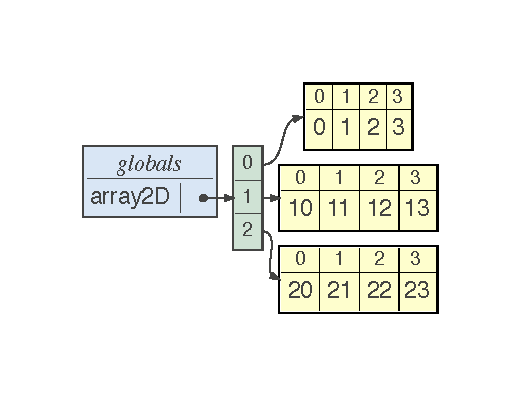
\includegraphics[width=\textwidth]{input/01-Clases-fig/Array2D}
\end{minipage}
\end{ejemplo}
Pero un array 2D no está obligado a que cada fila tenga el mismo número de columnas. Por ejemplo, la primera fila podría tener un valor, la segunda 10 valores, la tercera 5 valores, etc.

En este ejercicio deberá de implementar el TDA Array 2D usando el TDA Array 1D y con las siguientes especificaciones.


%%%%%%%%%%%%%%%%%%%%%%%%%%%%%%%%%%%%
%%%%%%%%%%%%%%%%%%%%%%%%%%%%%%%%%%%%
\input input/TDA-Array2D
%%%%%%%%%%%%%%%%%%%%%%%%%%%%%%%%%%%%
%%%%%%%%%%%%%%%%%%%%%%%%%%%%%%%%%%%%

Yo te construyo el método de inicialización y lo demás corre de tu cuenta:

\begin{pyverbatim}[][frame=single]
class Array2D:
  _the_rows: Array1D

  def __init__(self, *args: int):
    cols = tuple(args)
    rows = len(cols)
    assert rows > 0, "Array rows must be > 0 Excepcion"
    self._the_rows = Array1D(rows)
    for i in range(rows):
      assert cols[i] > 0, "Array cols must be > 0 Excepcion"
      self._the_rows[i] = Array1D(cols[i])
\end{pyverbatim}
Cuando en un método o función se usa \cm{*args} se está indicando que se considera una cantidad indeterminada de parámetros y que todos ellos serán empaquetados. Con el constructor indicado, se puede crear una instancia de Array2D indicando el número de columnas que tendrá cada fila. Por ejemplo, si se invocara como \pyv{array2D = Array2D(4, 7)} se construirá un array 2D cuya primera fila tendrá 4 elementos y la segunda fila tendrá 7 elementos.



%%%%%%%%%%%%%%%%%%%%%%%%%%%%%%%%%%%%%%%%%%%%%%%%%% 
\separacion
\section{Acceder a datos indexados} \label{sec:datosIndexados} 
\objetivo{1}{B}{Métodos de indexación \cm{[ ]}.}

Supón que construyes la clase Matriz con los atributos:

\hfil \pyv{._rows: int}, \pyv{._cols: int} y \pyv{._data: List[List[float]]}. 

Para acceder/modificar cierto elemento del array (usando POO) será necesario construir algunos métodos, que llamaremos \cm[black]{getItem(r: int, c: int) : float}, \cm[black]{setItem(r: int, c: int, v: float)} donde: \cm[black]{r} es la fila, \cm[black]{c} es la columna y \cm[black]{v} es el nuevo dato. Por ejemplo, para obtener el  elemento (2, 0) de la matriz se usará la notación punto de la forma \pyv{matriz.getItem(2, 0)}. Pero al trabajar con matrices ?`no sería deseable acceder con la notación indexada  \pyv{matriz[2, 0]} en vez de usar la notación punto? Sin duda para manipular datos indexados es más cómodo usar índices que usar métodos. 


\cm[red]{Python} permite acceder a elementos mediante índices si  la clase implementa los métodos mágicos \cm{\_\_getitem\_\_(self, index)} (para retornar el valor del índice dado) y 
\cm{\_\_setitem\_\_(self, index, value)} (para asignar un nuevo valor a la posición del índice dado). 

\begin{quotation}
En ambos métodos \cm{index} es una \textbf{tupla} que contendrá uno o varios números de tipo \pyv{int} que representará a los índices. En el caso de que \cm{index} tenga un solo índice se interpretará como un entero. 
\end{quotation}
 
La invocación a los métodos mágicos se hará con la escritura \cm[black]{objeto[i1, i2, ...]}, poniendo entre corchetes los índices. No confundir con la notación lista \cm[black]{iterable[i1][i2]...} de listas o tuplas.

Como ejemplos simples, suponiendo que las clases de los objetos que se indican ya tienen implementados los métodos mágicos adecuadamente:
\begin{itemize}
\item datos[4],  invocará a \cm{\_\_getitem\_\_(4)}  e \cm[black]{index} consta de un solo valor, el 4.
\item datos[4] = 20, invocará a \cm{\_\_setitem\_\_(4, 20)} e \cm[black]{index} consta de un solo valor.
\item matriz[2, 4],  invocará a \cm{\_\_getitem\_\_((2,4))}  e \cm[black]{index} consta de una tupla con dos valores.
\item matriz[2, 4] = 20, invocará a \cm{\_\_setitem\_\_((2, 4), 20)} e \cm[black]{index} será la tupla (2, 4).
\end{itemize}




Lo que se propone en este ejercicio es que en vez de  implementar los métodos \cm[black]{getitem()} y \cm[black]{setitem()} implementes los métodos \cm{\_\_getitem\_\_(self, index)} y \cm{\_\_setitem\_\_(self, index, value)} donde \cm{index} es una tupla. Una tupla es un tipo de dato similar a una lista pero es inumutable (ver \url{https://docs.python.org/3/library/stdtypes.html} para detalles). Implementados estos métodos podrá acceder al atributo que almacena todos los datos usando dos índices, donde el primero representa a la fila y el segundo a la columna.

\

Como ejemplo  de uso, el siguiente código debería funcionar:
\begin{pyverbatim}[][frame=single]
from TDAArray import Array2D

def main():
    # Building an array2D (4-rows and columns 2, 4 ,6, 2)
    mi_array = Array2D(2, 4, 6, 2)
    # Asignación de  datos  aleatorios
    for i in range(mi_array.num_rows()):
        for j in range(mi_array.num_cols(i)):
            mi_array[i, j] = (i+1)*10+(j+1)
    # Print data
    for value in mi_array:   # Check iterator
        print(value)

if __name__ == '__main__':
    main()
\end{pyverbatim}




Aplica esta técnica de indexación de datos siempre que puedas en tus propios tipos de datos (Array1D, Array2D, Matriz, ....). Es más \textbf{¿a que esperas para implementar estos métodos en los dos ejercicios anteriores? }






%%%%%%%%%%%%%%%%%%%%%%%%%%%%%%%%%%%%%%%%%%%%%%%%%% 
\separacion
\section{Matrices} \label{sec:MatrizDatosIndexados} 
\objetivo{2}{B}{Matriz con indexación \cm{[r,c]}.}


Construye la \textbf{clase Matriz} con los 3 atributos que se han indicado de tal forma que el siguiente código funcione. Las datos de la matriz se generan con el criterio que se desee. 

\begin{pyverbatim}[][frame=single]
m = Matriz(3, 6)
print(m[2, 0])  # __getitem__() retorna el dato (2, 0)
print(m)        # usar self[i, j] en __str__() para que imprima la matriz por filas
m[2, 0] = 100   # __setitem__() modifica el dato (2, 0)
print(m[2])     # __getitem__() retorna la fila 2
\end{pyverbatim}

Observa que para este ejercicio, \cm{\_\_getitem\_\_(self, index)} tendrá que analizar el caso en el que reciba uno (para retornar una fila) o dos enteros (para retornar un valor) .

%
%\
%
%
%\underline{\textbf{Enunciado antiguo - OBSOLETO}}
%Construya el TDA Array1D de acuerdo a lo indicado en la página \pageref{code:array1D}\footnote{Alternativamente puede construir la clase Array1D usando listas como arrays.} y cree la instancia \pyv{miArray = Array1D(3)}, entonces para acceder/modificar cierto elemento del array (usando POO) será necesario construir algún método, que llamaremos \cm[black]{getItem(index: int) : object}. Por ejemplo, para obtener el segundo elemento del array se usará la notación punto de la forma \pyv{miArray.getItem(1)}. Pero al trabajar con arrays ?`no sería deseable acceder con la notación indexada array \pyv{miArray[1]} en vez de usar la notación punto \pyv{miArray.getItem(1)}? Sin duda para manipular contadores indexados es más cómodo usar índices que usar métodos. Pues bien, \cm[red]{Python} permite acceder a elementos mediante índices si  la clase implementa los métodos  \cm{\_\_getitem\_\_(self, index)} y 
%\cm{\_\_setitem\_\_(self, index, value)}. Estos son dos de los muchos métodos que permiten definir operadores sobre objetos en Python. Puede ver todos los operadores que se pueden definir sobre una clase consulte \url{https://docs.python.org/3/library/operator.html}. 
%En particular, los dos que se indican nos permiten acceder a elementos del atributo (contenedor) \cm[black]{\_array} de la clase \cm{Array1D} usando índices. En concreto,  sobre la clase \pyv{class Array1D} se puede definir \cm{\_\_getitem\_\_()} de la siguiente forma:
%
%\begin{pyverbatim}[][frame=single]
%def __getitem__(self, index):
%  assert 0 <= index < len(self), "Array Index Out Of Bounds Exception"
%  return self._array[index]
%\end{pyverbatim}
%
%Una vez definido este método, se puede acceder a los elementos del contenedor del objeto  \pyv{miArray = Array1D(3)} usando la notación de índices \pyv{miArray[index]}. Cuando escriba \pyv{[index]}, entonces \cm[red]{Python} invocará al método \cm{\_\_getitem\_\_(index)} y en dicho método se accederá al \cm{index}-ésimo elemento del atributo \cm{\_array} (que es un array auténtico en \cm[red]{C} y usa notación indexada).
%
%\
%
%Complete la clase \pyv{class Array1D} para que tenga los siguientes métodos:
%\begin{itemize}
%\item Los métodos \cm{\_\_getitem\_\_()} y \cm{\_\_setitem\_\_()} para poder acceder y modificar los valores de una posición del atributo \cm{\_array} mediante un índice.
%El método \cm{\_\_getitem\_\_()} es el que ya tiene en el código anterior.
%
%\item El método \cm{clear()} que permite inicializar todos los elementos del arrays al valor dado.
%
%\item El método \cm{\_\_len\_\_()} que retorna la longitud del array (el valor de \cm{\_size}). Recordar que este método mágico es el que se invoca cuando se invoca a la función \cm{len()}.
%\end{itemize}
%
%Como ejemplo de uso, este código debería funcionar:
%\begin{pyverbatim}[][frame=single]
%size = 3
%miArray = Array1D(size)
%for i in range(len(miArray)):
%  miArray[i] = i*10
%for i in range(len(miArray)):
%  print(miArray[i])
%\end{pyverbatim}
%
%
%% - - - - - - - - - - - - - - - - - - - - - - - - - - - - - - - - - - - - - - - - - - - -
%
%%\input ejercicios/05-Funciones/AleatoriosSol.tex
%




%%%%%%%%%%%%%%%%%%%%%%%%%%%%%%%%%%%%%%%%%%%%%%%%%% 
\separacion
\section{Juego de la Vida}
\objetivo{2}{-}{Aplicación de Array 2D}


Un autómata celular bidimensional consiste en un array $n\times m$ donde cada celdilla (llamada célula) solo toma dos posibles valores, que indicaremos por \cm{False} (está muerta) y \cm{True} (está viva). En cada iteración las célula cambia su valor en función de los valores de las 9 células que la rodea en la iteración anterior. Se utilizan los siguientes criterios: 
\begin{enumerate}
\item Una célula muere  si dicha célula no tiene más de 1 vecino vivo o si tiene más de 3 vecinos vivo.

\item Se reemplaza una célula muerta por una viva si dicha célula tiene exactamente 3 vecinos vivos.

\item Una célula viva permanecerá en ese estado si tiene 2 o 3 vecinos vivos. 

\item Se considera que la frontera es periódica: las células de los bordes ``se unen'' con las células del borde opuesto (el array tiene forma de toro - ``donut'').
\end{enumerate}

Los autómatas celulares son modelos matemáticos y existen varios tipos. El que aquí se indica también se le llama Juego de la Vida y se puede estudiar su comportamiento usando el siguiente TDA.



\begin{definition}[TDA Juego de la Vida]{}\label{def:TDAJuegoVida}

El Juego de la Vida es un autómata celular que se representa en un grid o matriz $n\times m$.
Cada celda representa a un célula que puede estar viva o muerta de acuerdo a ciertas reglas de reproducción.

\begin{itemize}
\item \cm[black]{LifeGrid (nrows, ncols)}. Crea un array 2-dimensional que constará de \cm[black]{nrows}-índices fila y cada una tendrá y \cm[black]{ncols} columnas. Los argumentos tienen que ser positivos.


\item \cm[black]{numRows() : int}. Retorna el número de filas del grid.

\item \cm[black]{numCols(row) : int}. Retorna el número de columnas del grid.

\item \cm[black]{deadCell(i, j) : None}. Mata a la célula de la posición \cm[black]{(i, j)}.

\item \cm[black]{liveCell(i, j) : None}. Resucita a la célula de la posición \cm[black]{(i, j)}.

\item \cm[black]{isLiveCell(i, j) : boole}. Indica si la célula de la posición \cm[black]{(i, j)} está viva o no.


\item \cm[black]{numLiveNeighbors(i, j) : int}. Indica cuántas células vecinas de la posición 
\cm[black]{(i, j)} están vivas.

\item \cm[black]{evolve() : None}. Modifica todas las células del grid de acuerdo a las reglas de evolución.
\end{itemize}
\end{definition}

Obviamente, para su implementación tendremos un atributo que será un \cm[black]{Array2D} con lo que \textbf{tienen la obligación de utilizar} los métodos de esta clase. Así, por ejemplo, la implementación de \cm[black]{deadCell(i, j)} es simplemente invocar al método \cm[black]{setItem(i, j)} de \cm[black]{Array2D}. Tenga en cuenta en la implementación las particularidades de Python.


Como ejemplo de uso haga un programa que cree un juego de la vida y lo haga evolucionar 10 veces. Para ello implemente las funciones \cm{inicializar(automata: LifeGrid)} donde todas las células estén muertas menos las que considere y \cm{mostrar(automata: LifeGrid)} que muestre el estado del autómata en cada paso evolutivo.


% - - - - - - - - - - - - - - - - - - - - - - - - - - - - - - - - - - - - - - - - - - - -

%\input ejercicios/05-Funciones/CambioBaseSol.tex




%%%%%%%%%%%%%%%%%%%%%%%%%%%%%%%%%%%%%%%%%%%%%%%%%% 
\separacion
\section{Reversi}
\objetivo{3}{-}{Aplicación de Array 2D}

Reversi es un juego para dos jugadores sobre un tablero de $8\times 8$ celdas. Cada jugador tiene un número de fichas ilimitadas. Las fichas circulares tienen un color diferente en cada una de sus caras: por un lado es negra y por el otro lado es blanca. Un jugador juega a blancas - JugadorB - y otro jugador juega a negras - JuegadorN -. En cada turno se añade un ficha nueva y algunas fichas blancas del tablero pasarán a negras (si juega el jugadorN) o algunas fichas blancas del tablero pasarán a blancas (si juega el jugadorB). Cuando ya no se puedan poner fichas nuevas, ganará el jugador que tenga sobre el tablero más fichas de su color.

En cada turno, un jugador deberá de poner una ficha de su color en un celda. La celda tiene que cumplir que desde esa posición (1) deben existir en el tablero al menos una celda de su color en horizontal, vertical o diagonal, y (2) entre la celda donde se colocará la ficha y la otra celda del tablero deberán existir fichas del jugador contrario. Una vez colocada la ficha en la celda, se dará la vuelta a las fichas del jugador contrario que se encuentren entre la celda y la otra celda del tablero.
En el caso de que un jugador no pueda poner ficha porque no es capaz de encontrar una celda válida el turno pasa al otro jugador.
El juego finaliza cuando ninguno de los jugadores encuentran celdas válidas.


La configuración inicial del juego siempre empieza con 4 fichas ocupando las posiciones centrales y de la siguiente forma:

\hfil
{\footnotesize
\begin{tabular}{|c|c|c|c|c|c|c|c|} \hline
\phantom{o} & \phantom{o} & \phantom{o} & \phantom{o} & \phantom{o} & \phantom{o} & \phantom{o} & \phantom{o} \\ \hline
& & & & & & & \\ \hline
& & & & & & & \\ \hline
& & & \fullmoon & \newmoon & & & \\ \hline
& & & \newmoon  & \fullmoon & & & \\ \hline
& & & & & & & \\ \hline
& & & & & & & \\ \hline
& & & & & & & \\  \hline
\end{tabular}
}

Siempre empiezan las blancas, por lo que de acuerdo a las reglas de movimiento las celdas candidatas $\times$ se muestran a la izquierda. Si el JugadorB optara por la celda más superior, el tablero se modifica como se muestra a la derecha:

\hfil
{\footnotesize
\begin{tabular}{|c|c|c|c|c|c|c|c|} \hline
\phantom{o} & \phantom{o} & \phantom{o} & \phantom{o} & \phantom{o} & \phantom{o} & \phantom{o} & \phantom{o} \\ \hline
& & & & & & & \\ \hline
& &          &           & $\times$ & & & \\ \hline
& &          & \fullmoon & \newmoon & $\times$ & & \\ \hline
& & $\times$ & \newmoon  & \fullmoon & & & \\ \hline
& &          & $\times$  & & & & \\ \hline
& & & & & & & \\ \hline
& & & & & & & \\  \hline
\end{tabular}
}
{\footnotesize
\begin{tabular}{|c|c|c|c|c|c|c|c|} \hline
\phantom{o} & \phantom{o} & \phantom{o} & \phantom{o} & \phantom{o} & \phantom{o} & \phantom{o} & \phantom{o} \\ \hline
& & & & & & & \\ \hline
& & &           & \fullmoon & & & \\ \hline
& & & \fullmoon & \fullmoon  & & & \\ \hline
& & & \newmoon  & \fullmoon & & & \\ \hline
& & &           & & & & \\ \hline
& & & & & & & \\ \hline
& & & & & & & \\  \hline
\end{tabular}
}

A continuación se muestran las opciones del JugadorN y su movimiento final.

\hfil
{\footnotesize
\begin{tabular}{|c|c|c|c|c|c|c|c|} \hline
\phantom{o} & \phantom{o} & \phantom{o} & \phantom{o} & \phantom{o} & \phantom{o} & \phantom{o} & \phantom{o} \\ \hline
& & & & & & & \\ \hline
& & & $\times$  & \fullmoon & $\times$ & & \\ \hline
& & & \fullmoon & \fullmoon & & & \\ \hline
& & & \newmoon  & \fullmoon & $\times$ & & \\ \hline
& & &           & & & & \\ \hline
& & & & & & & \\ \hline
& & & & & & & \\  \hline
\end{tabular}
}
{\footnotesize
\begin{tabular}{|c|c|c|c|c|c|c|c|} \hline
\phantom{o} & \phantom{o} & \phantom{o} & \phantom{o} & \phantom{o} & \phantom{o} & \phantom{o} & \phantom{o} \\ \hline
& & & & & & & \\ \hline
& & &           & \fullmoon & \newmoon & & \\ \hline
& & & \fullmoon & \newmoon  & & & \\ \hline
& & & \newmoon  & \fullmoon & & & \\ \hline
& & &           & & & & \\ \hline
& & & & & & & \\ \hline
& & & & & & & \\  \hline
\end{tabular}
}

El juego continúa así hasta que no se puedan poner más fichas.

\

Se pide lo siguiente:

\begin{itemize}
\item Realiza  un proceso de abstracción para definir el TDA Reversi que contenga al menos los siguientes métodos: el constructor de juegos para tableros de tamaño $n \times n$ ($n \geq 4$ y par), el que inicializa un tablero, el que indica qué jugador gana, el que indica si una celda es un movimiento legal para un jugador, el que indica si una celda está ocupada, el que realiza un movimiento legal para un jugador.


Recuerda que los métodos son públicos, es decir, son los que se podrán usar desde otro módulo (p.e. un programa principal). Puedes construir métodos auxiliares (privados) para ciertos métodos públicos pero esos no se indican en el TDA.


\item Como ejemplo de uso, desarrolla un programa que permita al ordenador jugar contra sí mismo y tenga un función que permita mostrar en la consola la situación del tablero en cada turno.

Para que sea visible, hazlo para un tablero de $4\times 4$.
\end{itemize}

% - - - - - - - - - - - - - - - - - - - - - - - - - - - - - - - - - - - - - - - - - - - -

%\input ejercicios/05-Funciones/AreaRectangulosSol.tex
%
%
%
%
%\begin{ejercicio}
%\end{ejercicio}
%
%
%%%%%%%%%%%%%%%%%%%%%%%%%%%%%%%s%%%%
%%%%%%%%%%%%%%%%%%%%%%%%%%%%%%%%%%%
%\paragraph{Ámbito de una Variable.}
%
%
%
%
%
%% . . . . . . . . . . . . . . . . . . . . . . . . . . . . . . . . . . . . . . . . . . . . . . . . . . . . . . 
%\paragraph{Funciones Clausura.}
%%%%%%%%%%%%%%%%%%%%%%%%%%%%%%%%%%%%%%
%%%%%%%%%%%%%%%%%%%%%%%%%%%%%%%%%%%%%%
%{Funciones de Orden Superior: map()}
%
%\begin{itemize}[leftmargin=-.1in, rightmargin=-.3in]\setlength{\itemsep}{1mm}
%
%\item Podemos encontrar muchas funciones útiles sobre secuencias:
%
%\cm{map()}, \cm{filter()}, \cm{reduce()}, \cm{sum()}, \cm{len()}, \cm{any()}, \cm{all()}, \cm{min()}, \cm{max()}, $\ldots$ 
%
%\item Destacan las que \key{aplican un función sobre iterables}.
%	\begin{itemize}
%	\item Son funciones de orden superior
%	\end{itemize}
%	
%\item \cm{map(func, iter [, iter1, ..., iterN])}
%	\begin{itemize}
%	\item Retorna un iterador para \key{el resultado de aplicar} \cm{func} a los elementos de los \cm{iterables}.
%	
%	\item \cm{func} es la función por la que pasan los elementos de los iterables.
%	
%	La función puede ser una función lambda.
%	
%	\item \cm{iterK} son los iterables que serán 'mapeados'.
%	
%
%	\textbf{Ejemplo:} ?`Cómo sumar los valores de dos listas?
%
%
%
%\begin{pyconsole}[][frame=single, fontsize=\scriptsize]
%lista1 = [1, 2, 3, 4]
%lista2 = [5, 6, 7, 8, 9, 10]
%# Modo tradicional
%sol = []
%for i in range(len(lista1)):
%  sol.append(lista1[i] + lista2[i])
%
%sol # sol es una lista
%\end{pyconsole}
%
%
%\begin{pyconsole}[][frame=single, fontsize=\scriptsize]
%# Modo 1
%def suma (x, y):
%    return x + y
%
%sol = map(suma, lista1, lista2)
%# Modo 2
%sol = map(lambda x, y: x+y, lista1, lista2)
%
%list(sol)   # sol es un objeto map.
%\end{pyconsole}
%
%
%
%		\end{itemize}
%
%\end{itemize}
%
%
%
%
%\centerline{\Large \bf Ejercicios}
%
%\
%
%\formatoEjercicio


